\newcommand{\darmerr}{\texttt{DARM\_ERR} }

As discussed in section \ref{sec:detection_statistics}, the CBC group
measures the significance of candidate events by comparing the
combined new SNR (eqn.~\ref{eq:new_snr}) against the background
distribution.  The background is obtained by sliding the triggers from
each IFO against each other by more than the light travel time between
them.  In the limit of at most one real gravitational wave in each
analysis segment this ensures that the background is composed entirely
of triggers resulting from non- gravitational-wave sources.

Ideally, the instrumental noise would be Gaussian and the only source
of extraneous triggers would be random fluctuations.  In reality
environmental couplings to the instrument, such as electrical and
seismic, as well as glitches within the instrument will also produce
triggers.

It is in the interest of the collaboration to remove as many of these
triggers as possible so that any real events will stand out well above
the background.  This removal must be done in an automated way in
advance of looking at the results from the analysis.  The LIGO and
Virgo collaborations would be justly criticized if the background were
to be adjusted after the analysis in order to make a marginal
candidate appear more significant.

There is therefore a need for a process of detector characterization
(henceforth ``detchar''), a way to remove times from the analysis that
are more likely to produce triggers from noise than from a real event.
One of the most significant features of the S6 run is that the people
working on detchar were in close contact with the people commissioning
the instrument.  This meant that, in addition to cleaning the search,
information about problematic behavior in the instrument could be used
to fix the problems at the source, in turn allowing more time to be
analyzed and the prospects for making a detection to improve.

Detchar was a major undertaking, much more information can be found in
(Smith and Lundgren in progress).  Three primary tools were run
continuously or with low-latencies to provide views into the data,
although these were supplemented with numerous short special-purpose
scripts.  Two of these tools, the klinewelle pipeline~\cite{} and the
Omega pipeline~\cite{} project data onto a wavelet basis and identify
as triggers times and frequencies with amplitudes above a given
threshold.  Both these tools were run on many auxiliary channels in
addition to the detector output.  The third tool, daily ihope, is the
focus of the current chapter.


\section{Daily ihope}

As discussed in (search chapter) the CBC group uses the \emph{ihope}
pipeline to search for gravitational waves produced by the inspiral of
binary systems consisting of neutron stars and/or black holes.  During
LIGO's 6th science run (July 7, 2009 - October 20, 2010) which
overlapped Virgo's second (July 7, 2009 - January 11, 2010), and third
(August 11, 2010 - October 20, 2010) science runs, the goal of the
group was to run the full analysis every two weeks with latencies as
small as possible.  The daily ihope runs were conceived of as a way to
characterize the detector in order to look for potential problems in
advance of the full search, particularly problems specific to the CBC
search.

It is important to stress that daily ihope was not itself a
gravitational wave search, it was a tool to help determine whether the
data in each instrument was suitable to analyze.  This goal determined
the specifics of the daily runs, but more significantly it leaves the
full search unbiased.

\subsection{The Daily Ihope Pipeline}

Recall that ihope is a templated, matched-filter search.  For the
low-mass search, which was the focus of the daily runs, the templates
are restricted, stationary-phase frequency-domain waveforms with phase
evolution taken to 3.5 PN order.  The templates are laid out in a bank
with 97\% overlap between nearest neighbors, and the mass range is
from 2 $\msun - 25 \msun$.  A $\chisq$ discriminator is constructed to
better separate signals from glitches (eqn.\ref{eq:chisq}), and the
information from this discriminator is used along with the SNR to
construct the new SNR detection statistic (eqn.~\ref{eq:new_snr}).

By construction, a great deal of the information provided by
the full bank search is redundant.  Further, the evaluation of each
additional template and the initial layout of the bank incurs
significant computational overhead.  Therefore a number of
simplifications were applied to the daily ihope bank.

First, a static bank was used for each IFO, based on the layout at a
time in each instrument when the inspiral range was high, no
operational problems were noted by the scimon or operator, and the
Omega, KW, and daily ihope pipelines showed no anomalous behavior.
Second, the number of templates was reduced.  Lower-mass systems have
more cycles in the sensitive LIGO band, there is therefore ample
information to distinguish between waveforms with close parameters.
Conversely, this means that the low-mass end of the bank is very dense
(in the sense of number of templates per unit square in parameter
space, they are still equidistant in the sense of the bank metric.
Such fine resolution is not needed when looking for glitches,
therefore the minimal match between templates in the region below a
chirp mass ($\mathcal{M} = M \eta^{3/5}$) of 3.46 $M_\odot$ was set to
0.5.  At higher masses, up to a total mass of $25 M_\odot$, the
minimal match was set to 0.95.  In addition to ensuring coverage in a
mass region which is naturally sparser this ensures that short
glitches, characteristic of many glitch mechanisms, were flagged with
large SNRs.  The resulting hybrid bank for the Hanford detector is
shown in figure \ref{f:daily_ihope_bank}.

\begin{figure}
  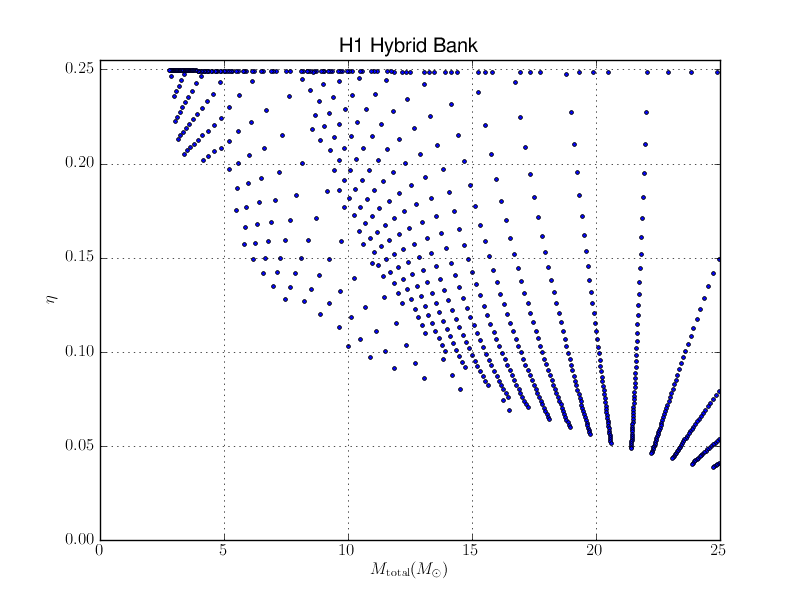
\includegraphics[width=\linewidth]{figures/detchar/hybrid_bank.png}
  \caption[The hybrid template bank used by daily ihope]{
  \label{f:daily_ihope_bank}
The hybrid template bank used by daily ihope for the Hanford detector,
the banks for L1 and V1 are similar.
The cut is made at constant chirp mass, which is
a curve in the total mass, $\eta$ plane.}
\end{figure}%

Daily ihope processing ran at 03:00 GMT and examined data spanning the
24 hours ending at 00:00 GMT.  Unlike full ihope, the analysis was
done on all science time, including that which would be vetoed at CAT
1 by the full analysis.  This was done so that we could see the effect
of the CAT 1 vetoes.  It is plausible, for example, that some such
vetoes would be too aggressive and we could decide based on the daily
results to include such times back into the analysis.  For consistency
science time was denoted CAT 0.  In addition CAT 3 vetoes to remove
hardware injections were not applied, so that we could see how many
injections would be lost by CAT 4 vetoes.  The daily pages therefore
displayed results for categories 0, 1, 2, and 4.

For each 2048-second chunk of contiguous data, at each IFO, the data
was run through each template in the bank and triggers selected as
described in section \ref{sec:analysis_trigger_selection}. For each
trigger $\chisq$ and new SNR were calculated and recorded.  Clustering
was then done in order to focus attention on glitches that were most
likely to cause problems in the full search.  Two sets of clustered
triggers were recorded using windows of 30 milliseconds and 16
seconds.  For each set the trigger with the largest value of new SNR
across all templates within the window length was recorded.

The triggers were also filtered.  A version of the veto definer file
designated as ``online'' was maintained and used by daily ihope to
identify times with veto categories.  These vetoed times were then
removed from the original and clustered files.  
% The pipeline is summarized in figure (xx).
The result is, for each 2048-second block in each ifo, 3 cluster
levels times 4 veto levels = 12 sets of triggers.

The structure of the daily pipeline is shown in figure \Note{make
this}.  For comparison we include the structure of the full search,
shown in figure~\ref{f:hipe}~\footnote{Figure by Collin Capano, used
with permission}.  We will not go over it in detail here, but note
that it is a two-stage, coincident pipeline.

\begin{figure}
  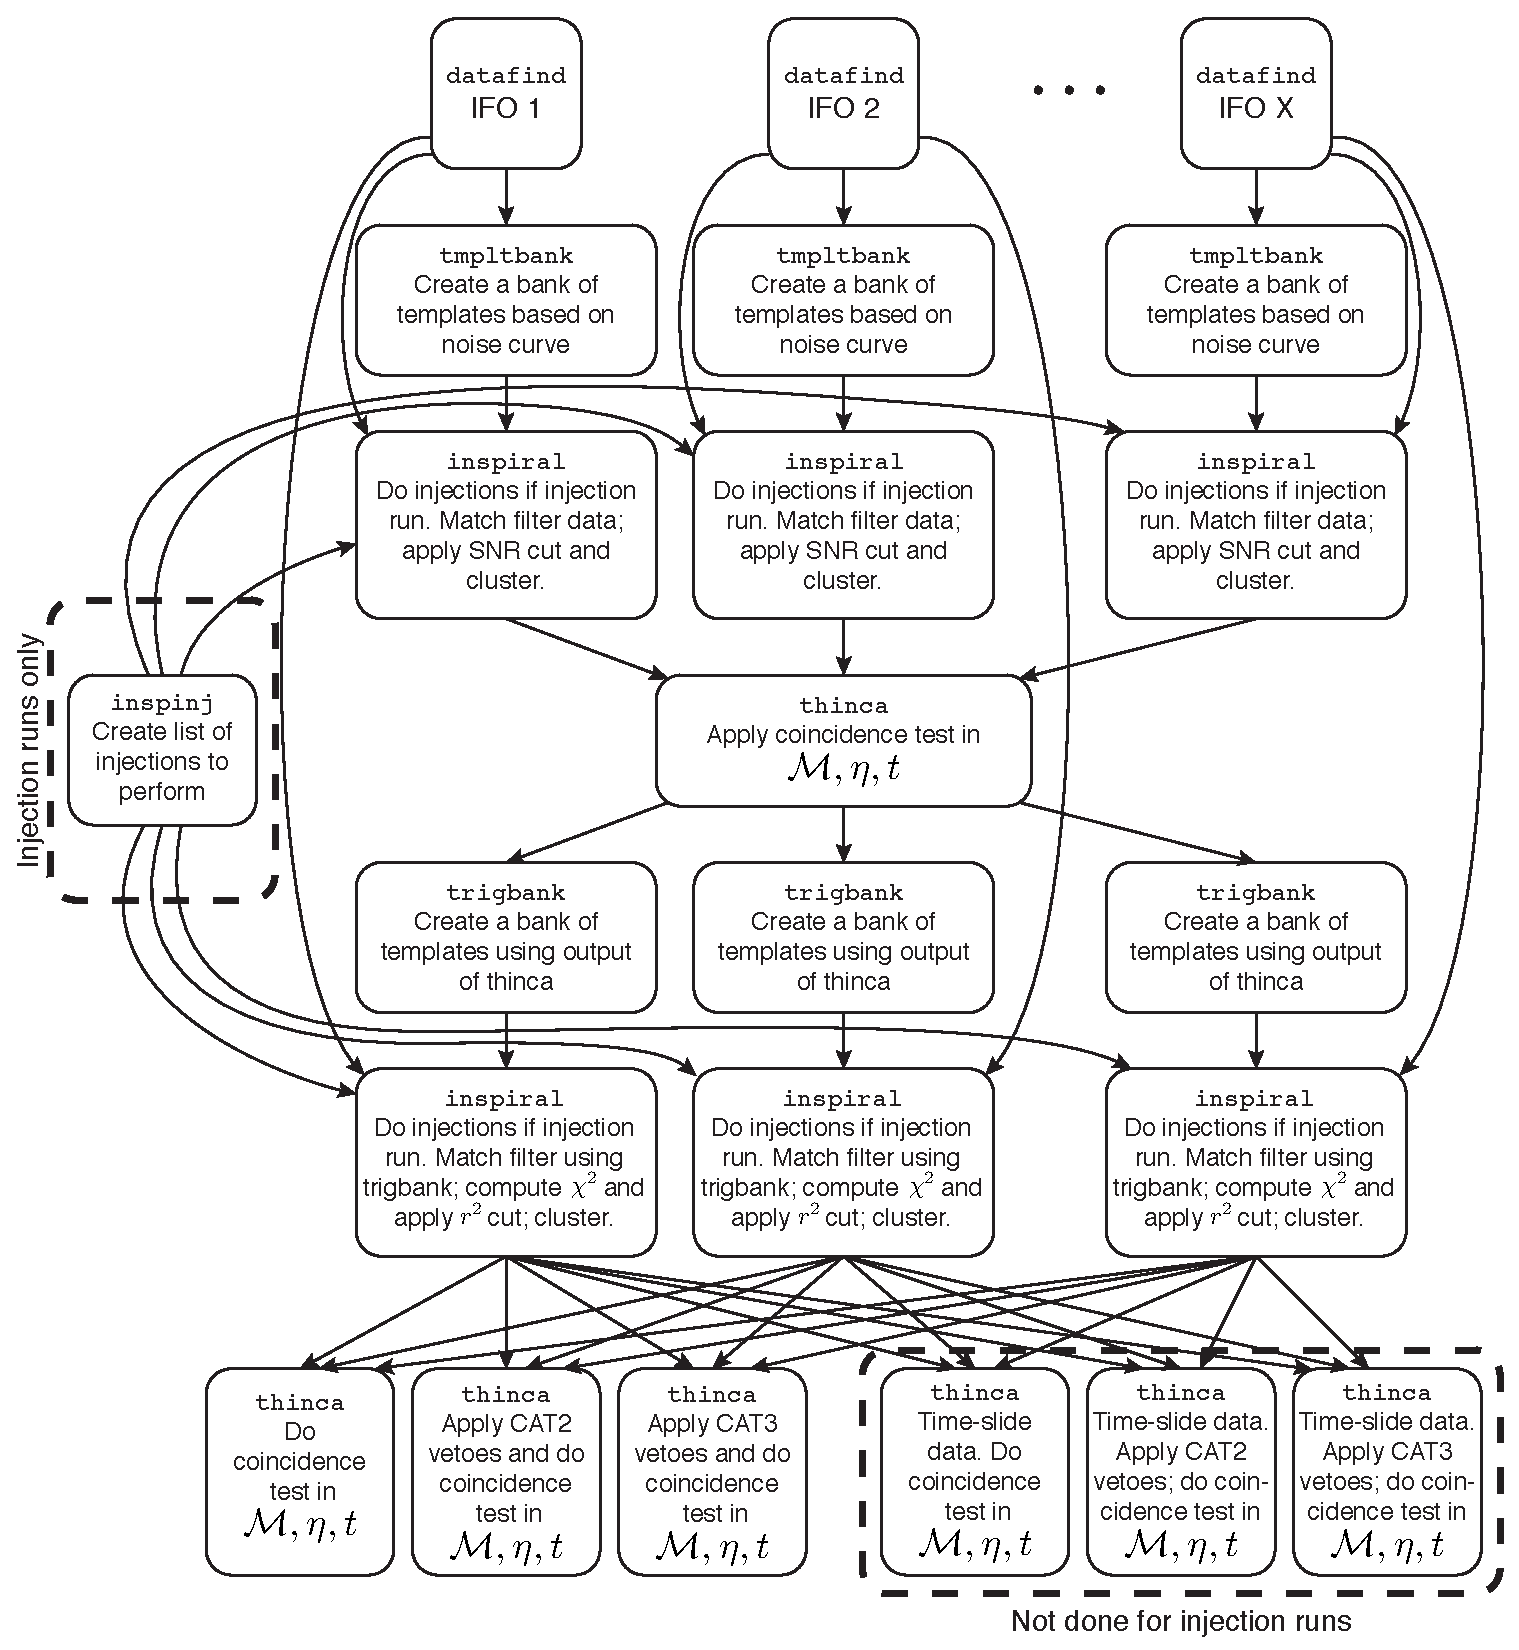
\includegraphics[width=\linewidth]{figures/detchar/HIPEDiagram}
  \caption[Structure of the full iHope search]{
  \label{f:hipe}
Structure of the full iHope search.  For details see (\Note{Collin's
thesis}).
}
\end{figure}%

%do analysis
%record science triggers
%cluster 30 ms     determine cat 1
%cluster 16 sec    determine cat 1 + cat 2
%                  ...

%filter and record

\section{The Daily Ihope report pages}

Much of the utility of the daily runs was in the use of the resulting
triggers to identify data quality issues and quantify the value of
proposed vetoes.  Some of these uses will be discussed in
section~\ref{sec:applications_vetoes}.  In addition to the triggers
the daily pipeline also produced a large number of plots and reports,
organized into web pages that were available to the collaboration.
Data analysts could use these pages to spot potential problems for the
full analysis and begin more detailed followup studies.  

We now summarize the contents of the daily pages. Each report and plot
is made for each combination of the following:

\begin{itemize}
\item IFO: H1, L1 and V1
\item Cluster level: Unclustered, 30 ms clustering, 16 second
clustering
\item Veto level: Show all triggers in science time (level ``0''),
only those not removed by category 1 vetos, only those not
removed by categories 1 or 2, or only those note removed by
categories 1,2 and 4.  Hardware injections vetos (category 3) were not 
applied so that we could determine whether category 4 vetoes were 
remove them.
\end{itemize}

Each of these features could be set independently.  The top-level web
interface for a sample day is shown in figure~\ref{f:daily_ihope_top}.

\begin{figure}
  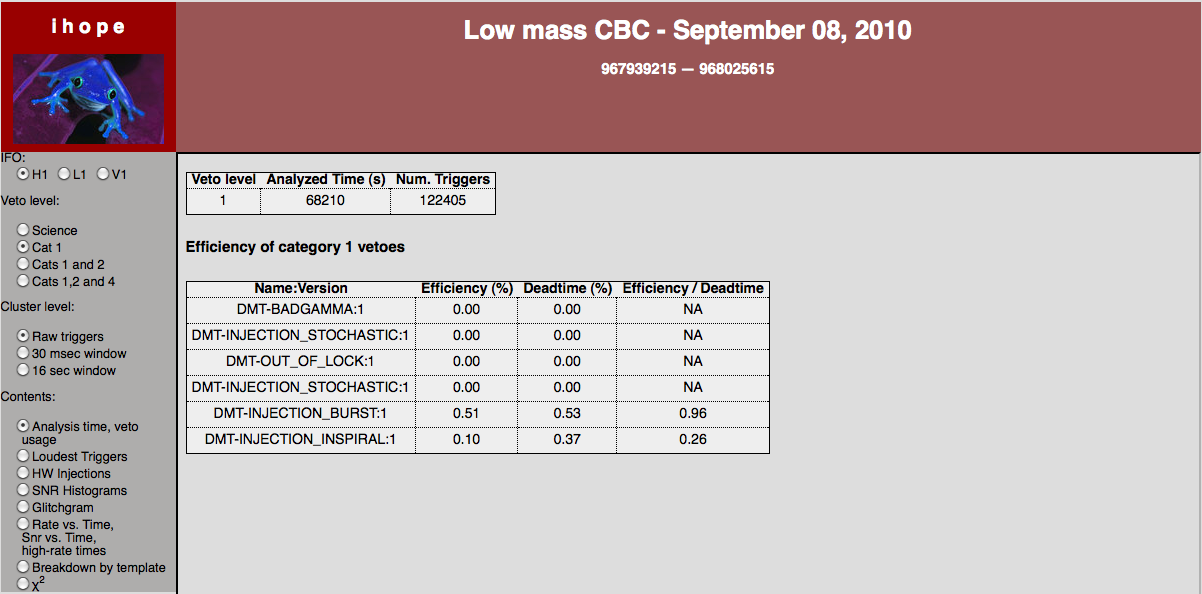
\includegraphics[width=\linewidth]{figures/detchar/daily_ihope_top}
  \caption[Top-level web interface for daily ihope]{
  \label{f:daily_ihope_top}
Top-level web interface for daily ihope.  Options can be selected with
the controls on the left hand side, when a button is clicked the
contents region is immediately replaced.  The default view is the one
shown here; the analysis time and veto efficiency at cat 1 for the
Hanford detector.}
\end{figure}%

The available reports can bee seen at the bottom of the list of
controls in figure~\ref{f:daily_ihope_top}:

\weakheader{1. Analysis time and veto usage.}

This report shows the total time analyzed, the vetoes applied beyond
those applied at the previous level, the \emph{efficiency} (percentage
of triggers removed) and \emph{deadtime} (percentage of time removed)
by each veto.  In addition the ratio of efficiency over deadtime is
reported as a measure of quality of the veto.  A random veto would
result in an efficiency-over-deadtime of approximately 1, a
finely-tuned veto that removes short, loud events that ring off the
entire template bank would have a much higher ratio.   An example is
shown in figure~\ref{f:daily_ihope_vetousage}.


\begin{figure}
  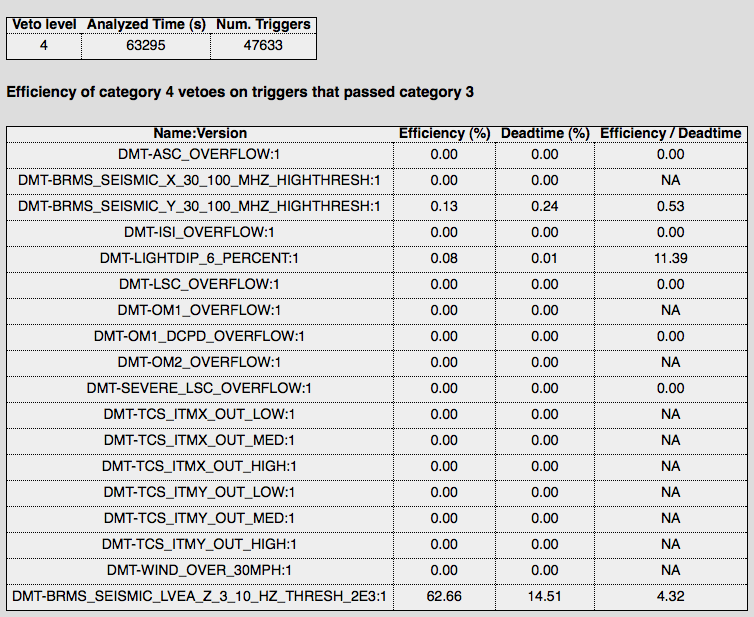
\includegraphics[width=\linewidth]{figures/detchar/vetousage.png}
  \caption[Sample veto usage report from Aug 19, 2010]{
  \label{f:daily_ihope_vetousage}
A sample veto usage report, see text for explanation.  Note that 62.66\% of
all triggers were contained in 14.51\% of time, and the DMT flagged this time
with elevated seismic activity from 3-10 Hz at the LVEA.}
\end{figure}%

\weakheader{2. Loudest triggers}

This report was only run for 16-second-clustered triggers.  Loud
glitches tend to produce families of triggers, without clustering the
loudest triggers from each day would likely result from one underlying
event.  This report considers two classes of triggers; those where no
data quality flag was active and those where at least one flag was
active.  A sample report is shown in
figure~\ref{f:daily_ihope_loudest}.  For the five triggers with
highest new SNR in each category a summary was presented along with a
link to an \emph{omega scan}.  The omega pipeline is described in
(\checkme{omega refs}).  Omega scans are a kind of time-frequency
plot.  They are especially useful as they may be run on all auxiliary
channels recorded by the instruments and therefore provide a visual
aid to detecting coupling between auxiliary channels and the
gravitational wave readout channel.  These can be used to suggest
mechanisms behind glitches, especially those that were not already
marked by a DQ flag.  In addition, over time repeated shapes in the
omega scan can pinpoint underlying problems in the instruments that
need to be addressed.  A few images from one of the glitches in
figure~\ref{f:daily_ihope_loudest} is shown in
figure~\ref{f:daily_ihope_loudest_omega}.

\begin{figure}
  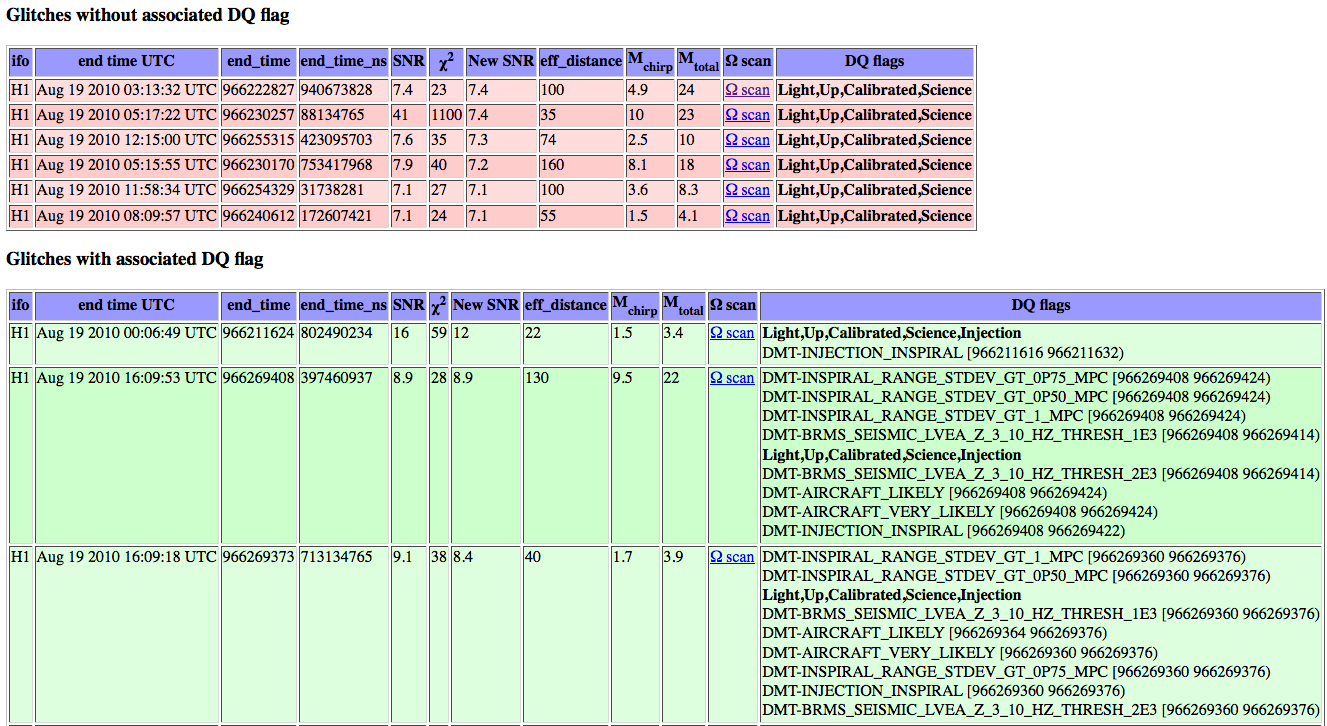
\includegraphics[width=\linewidth]{figures/detchar/loudest.png}
  \caption[Sample loudest trigger report from Aug 19, 2010]{
  \label{f:daily_ihope_loudest}
A sample report on loudest triggers, see text for explanation.  Note the
rightmost column is populated by
the \texttt{ligolw\_dq\_query} program in the \texttt{--report} mode.}
\end{figure}%



\begin{figure}
  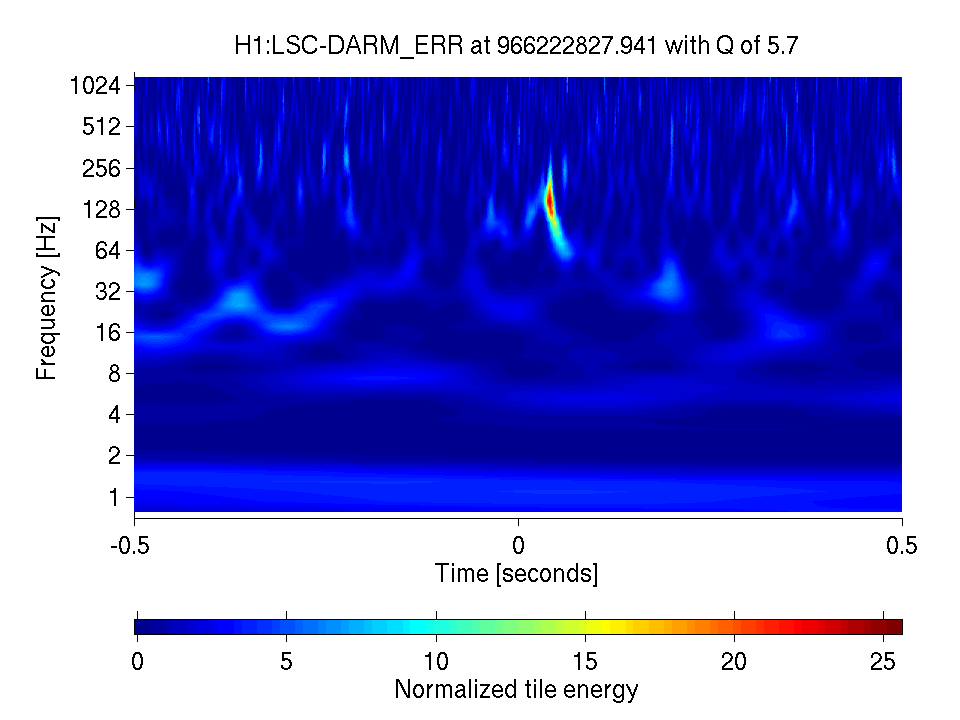
\includegraphics[width=0.5\linewidth]{figures/detchar/966222827_940673828_H1_LSC-DARM_ERR_1_00_spectrogram_whitened.png}
  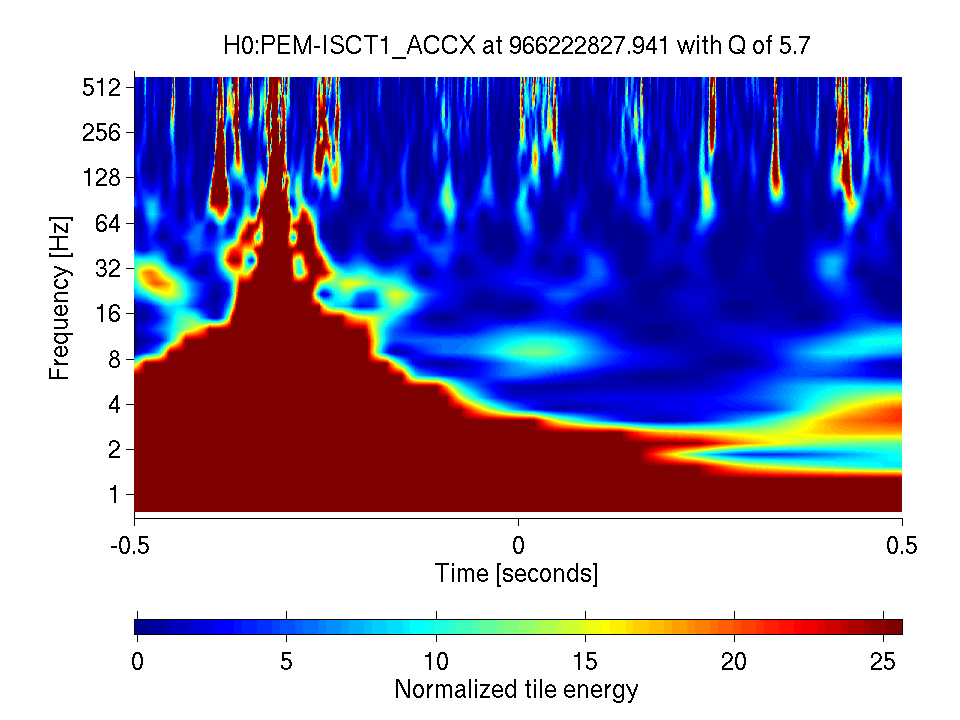
\includegraphics[width=0.5\linewidth]{figures/detchar/966222827_940673828_H0_PEM-ISCT1_ACCX_1_00_spectrogram_whitened.png}
  \caption[Omega scans from the loudest H1 trigger in figure \ref{f:daily_ihope_loudest}]{
  \label{f:daily_ihope_loudest_omega}
Omega scans from the loudest H1 trigger in figure
\ref{f:daily_ihope_loudest}.
Note the trigger closely follows a loud
event in one of the accelerometers on an instrument table.}
\end{figure}%


\weakheader{3. Hardware injections}

This report was generated by code written by John Veitch  at Cardiff
University.  It compared the list of injections, published as an XML
file available from a web site, with the list of analysis times and
triggers.  The results were plotted to indicate whether each injection
was found, missed, or not analyzed.


\weakheader{4. SNR histograms}

These plots show the number of triggers as a function of SNR and new
SNR.  As noted in section \ref{sec:ihope_match_filter}, in Gaussian
noise the number of triggers should be proportional to
$\exp(-\rho^2/2)$.  These plots therefore show the degree of
``non-Gausianity'' in the data.  A common use for these plots was to
flip between veto levels to get a sense of how well the cumulative
vetoes were cleaning the data, as shown in figure
\ref{f:daily_ihope_gaussianity}.

Similarly figure~\ref{f:daily_ihope_gaussianity_newsnr} shows histograms
of the triggers in new SNR.  The total number of triggers is greatly
reduced because many high-SNR triggers have $\newsnr < 5$ , where the
plot cuts off.  While triggers with such low $\newsnr$ values are not
excluded from later stages of analysis in the full pipeline, it is
extremely unlikely that the resulting combined new SNR will be high
enough to stand above background.

In addition to the lower number of triggers overall, the new SNR plot
is closer to a straight line indicating behavior closer to that
expected in Gaussian noise.  However, detchar improves the situation
still further, as the number of triggers is reduced at veto category
4.

However, there is one trigger with $\newsnr = 8$ that is not removed
by any veto.  Such an outlier warrants further investigation, which
here is provided by the loudest events page an example of which is
shown in~\ref{f:daily_ihope_loudest}.  The omega scan from the time of
this event is shown in figure~\ref{f:daily_loudest_glitch}, and it
clearly rules out a gravitational wave as the source of this trigger.
This illustrates the important point that new SNR can be fooled, and
hence continued human participation in detchar is necessary.

\begin{figure}
  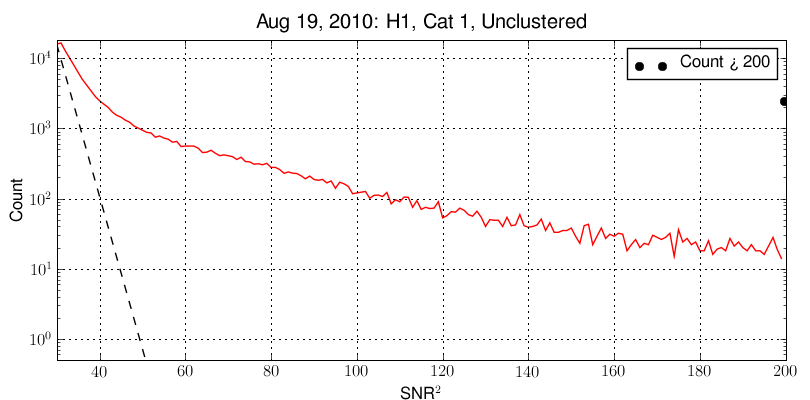
\includegraphics[width=0.5\linewidth]{figures/detchar/H1_1_UNCLUSTERED_snr_hist.png}
  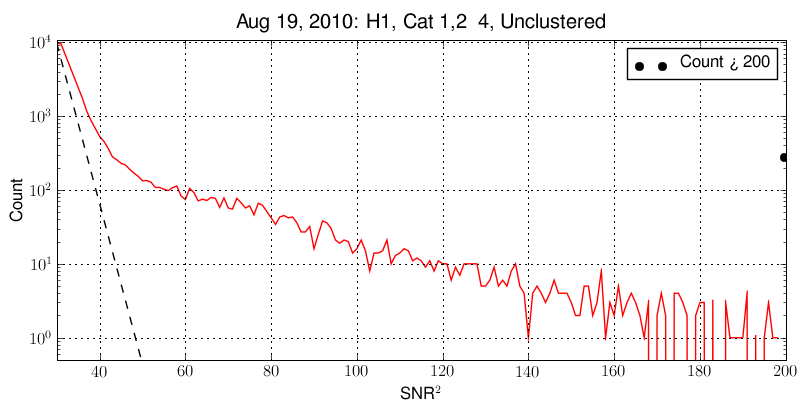
\includegraphics[width=0.5\linewidth]{figures/detchar/H1_4_UNCLUSTERED_snr_hist.png}
  \caption[Trigger SNR histograms for H1]{
  \label{f:daily_ihope_gaussianity}
Sample trigger histograms by SNR.  The dashed line shows the
expected values in Gaussian noise.  The dot indicates the cumulative
number of triggers with new SNR greater than 200.  Note that at veto
category 4 (right) the histogram is closer to the expected line than
it is at category 1 (left).  This indicates the degree to which data
quality has removed non-Guassian noise.}
\end{figure}%



\begin{figure}
  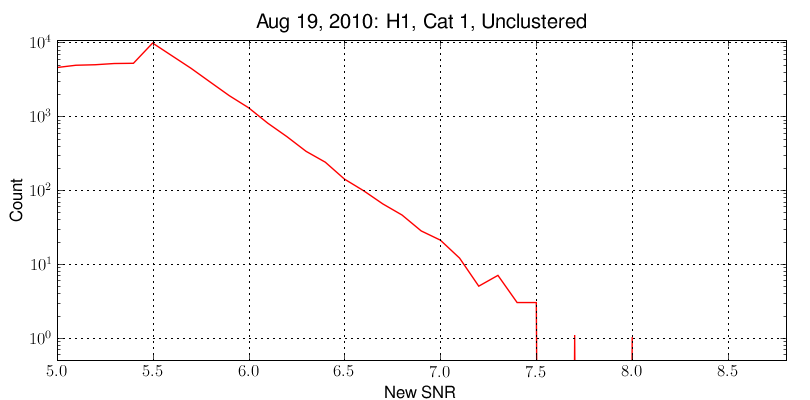
\includegraphics[width=0.5\linewidth]{figures/detchar/H1_1_UNCLUSTERED_new_snr_hist.png}
  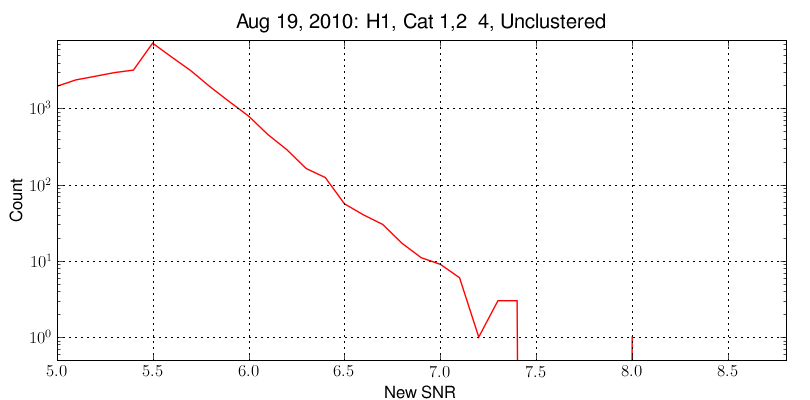
\includegraphics[width=0.5\linewidth]{figures/detchar/H1_4_UNCLUSTERED_new_snr_hist.png}
  \caption[Trigger new SNR histograms for H1]{
  \label{f:daily_ihope_gaussianity_newsnr}
Sample trigger histograms by new SNR. The data is much cleaner than
the SNR histograms, but there is still an outlier at $\newsnr=8$.}
\end{figure}%



\begin{figure}
  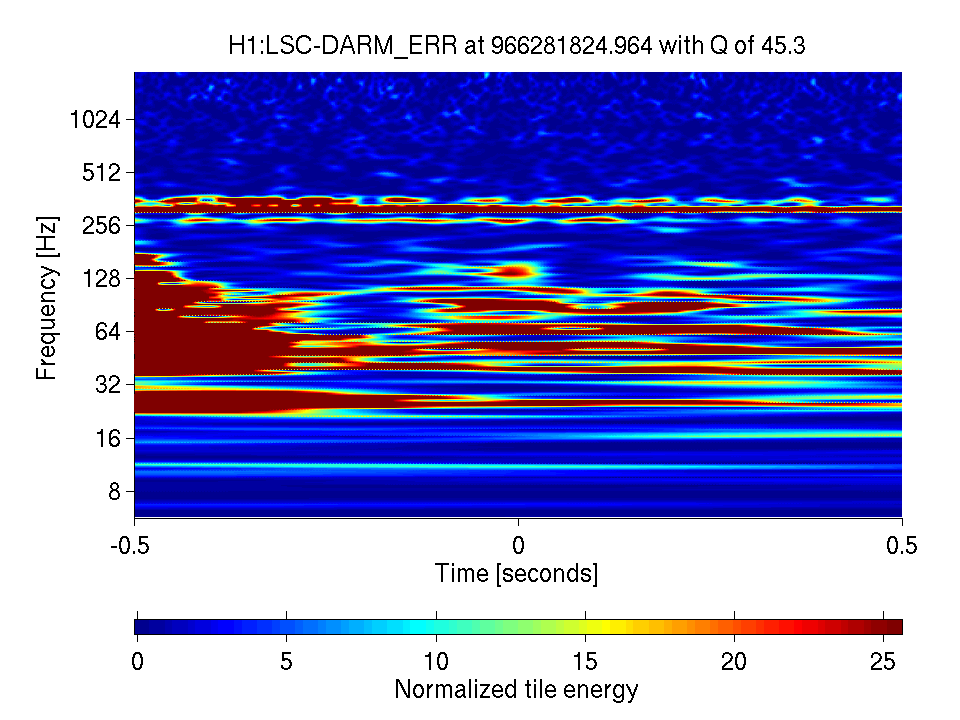
\includegraphics[width=\linewidth]{figures/detchar/966281824_963867187_H1_LSC-DARM_ERR_1_00_spectrogram_whitened}
  \caption[Omega scan of the loudest new SNR trigger]{
  \label{f:daily_loudest_glitch}
The omega scan from the outlier with new SNR=8 that survives all
automated data quality vetoes.  Many auxiliary channels showed the
same behavior at this time.  This is clearly not a gravitational wave,
but was not removed by either signal-based vetoes or data quality
vetoes.}
\end{figure}%


\weakheader{5. The ``glitchgram''}

This was an ``at-a-glance'' summary of the day, showing every trigger
color-coded by SNR.  This highlighted times of loud triggers as well
as dense regions indicating ``grumbly'' times.  A sample is shown in
figure \ref{f:daily_ihope_glitchgram}.

\begin{figure}
  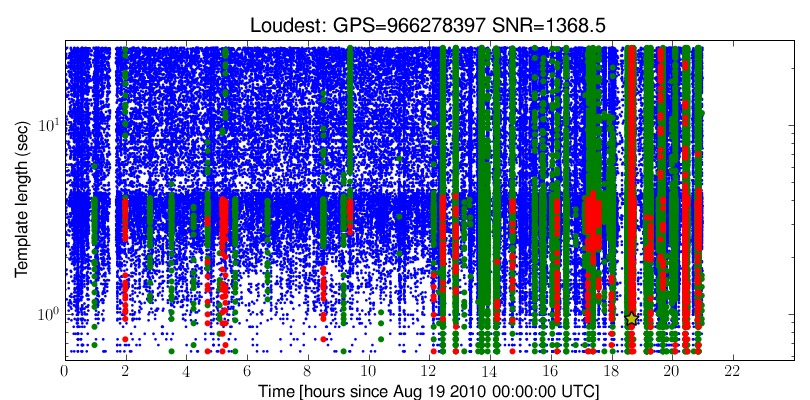
\includegraphics[width=\linewidth]{figures/detchar/H1_1_UNCLUSTERED_glitchgram.png}
  \caption[The Aug 19th daily ihope ``glitchgram'']{
  \label{f:daily_ihope_glitchgram}
A sample ``glitchgram.'' Blue dots have
new snr values below 8, green have values between 8 and 16,
and red have values above 16.  Template length was chosen as the Y
axis in order to capture a feature of the templates that is not
specific to gravitational wave signals, such as chirp mass.
Note the break at 4.3 seconds, corresponding to the
chirp mass at which the bank switches from an overlap of 0.95 to 0.5.
Comparing to figures 3 and 4 shows the same 
excess of triggers after 12:00.  No data is analyzed after 21:00
because ihope requires at least 2048 contiguous seconds to estimate
the PSD and all data after this time was in smaller segments.}
\end{figure}%


\weakheader{6. Rate vs. Time and SNR vs. Time}

These plots complimented the glitchgram by breaking the triggers up
differently.  The rate plot (figure~\ref{f:daily_ihope_rate_v_time})
showed average number of triggers over 1-minute intervals.  The SNR
plot (figure~\ref{f:daily_ihope_snr_v_time}) showed the SNR of every
trigger as a function of time.  These tend to be correlated, as loud
glitches ring off the entire bank and produce large numbers of
triggers.  The plots were accompanied by tables showing the times
where the rate of triggers exceeded 500 Hz for more than one second,
and exceeded 200 Hz for more than 10 seconds.

\begin{figure}
  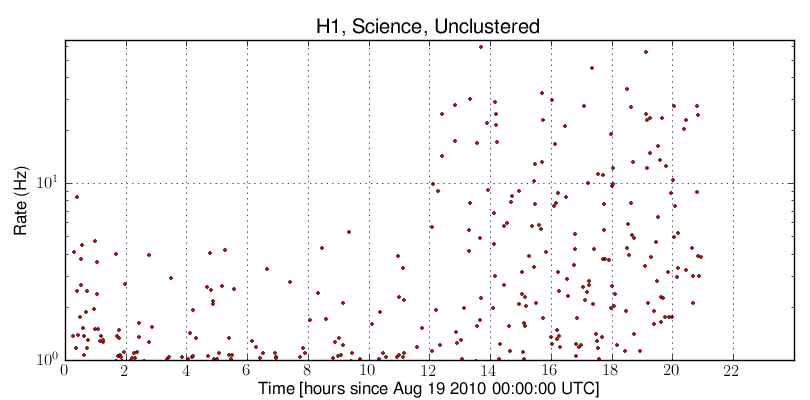
\includegraphics[width=\linewidth]{figures/detchar/H1_0_UNCLUSTERED_rate_vs_time.png}
  \caption[Daily ihope rate plot]{
  \label{f:daily_ihope_rate_v_time}
Sample rate plot, showing rate in Hz (averaged over
1-minute intervals) as a function of time.  Note that the rates
increase after 12:00.  This was due to increased seismic noise.}
\end{figure}%

\begin{figure}
  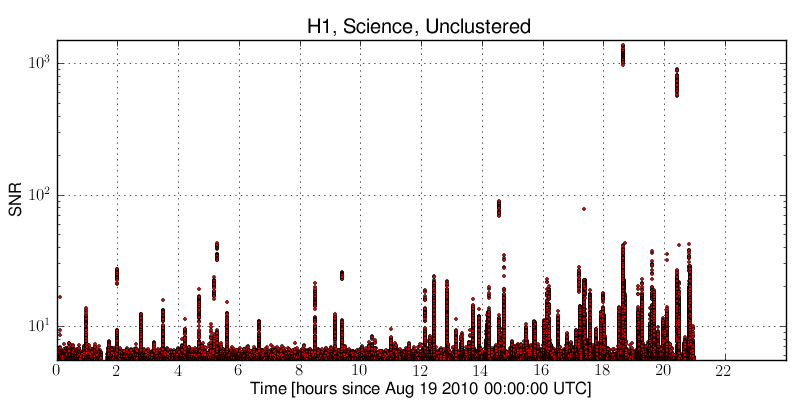
\includegraphics[width=\linewidth]{figures/detchar/H1_0_UNCLUSTERED_snr_vs_time.png}
  \caption[Daily ihope SNR plot as a function of time]{
  \label{f:daily_ihope_snr_v_time}
Sample plot of SNR as a function of time.  The density of
triggers increases somewhat after 12:00 and there are more loud
outliers.  However the change in behavior is better seen in 
figure \ref{f:daily_ihope_rate_v_time}.}
\end{figure}%


\weakheader{7. Breakdown by template}

This page showed several histograms of number of triggers as a
function of the length of templates in seconds.  Examples of the
standard histograms are shown in
figure~\ref{f:daily_ihope_trig_histograms}, they show that most of the
triggers come from short templates, and templates shorter than 5
seconds produce up to six times as many triggers as shorter templates.

Figure~\ref{f:count_per_template} shows the same information as a map
of the template bank, color-coded to indicate how many triggers each
template produced.  Figure~\ref{f:daily_ihope_time_mass} breaks this
same information up by time and template mass.

Qualitatively these plots do not change much day-by-day, and so these
plots were not often used.  However, they did prompt a change to
the analysis made early in the S6 run, see
section~\ref{sec:applications_pipeline}.

\begin{figure}
  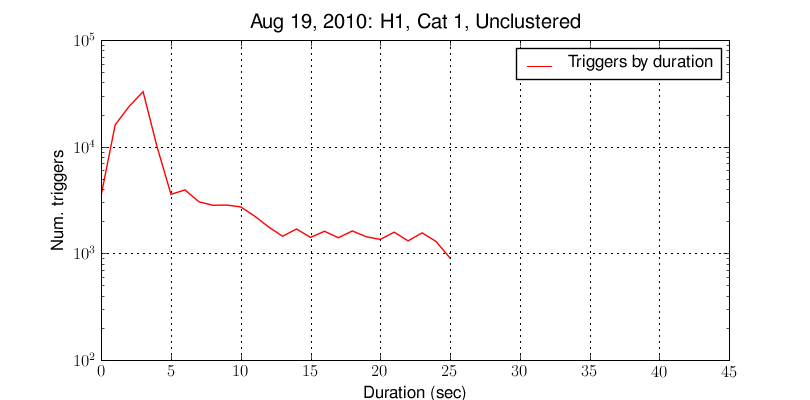
\includegraphics[width=0.5\linewidth]{figures/detchar/H1_1_UNCLUSTERED_mass_hist}
  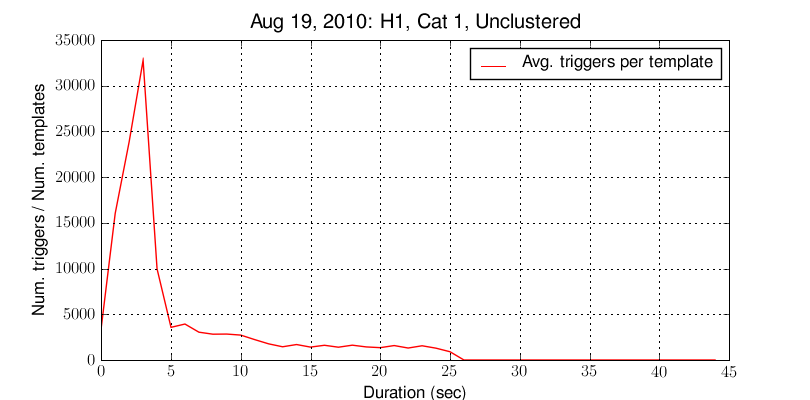
\includegraphics[width=0.5\linewidth]{figures/detchar/H1_1_UNCLUSTERED_mass_hist_norm}
  \caption[Histograms of trigger rates by template length]{
  \label{f:daily_ihope_trig_histograms}
Histograms of trigger rates by template length in daily ihope.  The
plot on the left combines all templates, the plot on the right
normalizes by plotting (number of triggers resulting from templates of
length $x$) divided by (number of templates of length $x$).
}
\end{figure}%

\begin{figure}
  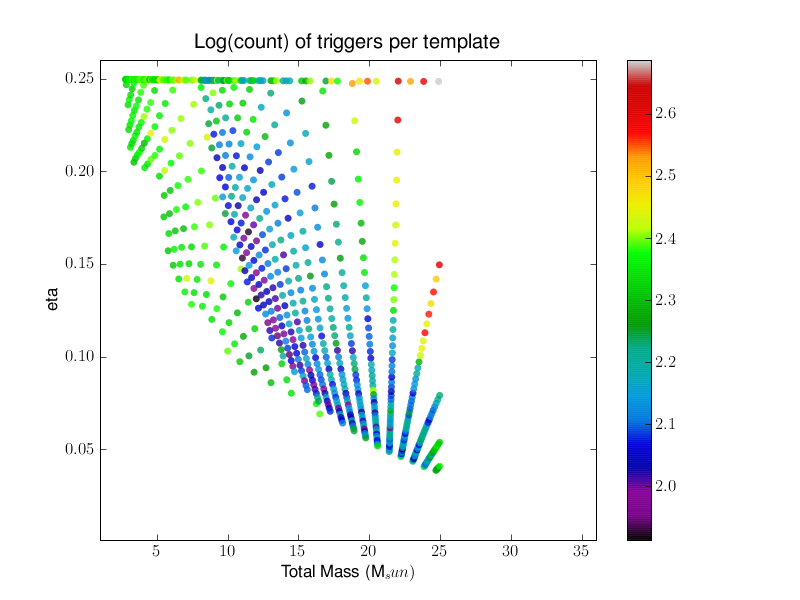
\includegraphics[width=\linewidth]{figures/detchar/H1_1_UNCLUSTERED_template_counts}
  \caption[Triggers per template]{
  \label{f:count_per_template}
The daily template bank, color-coded to show how many triggers each
template produced.  Note that the template in the upper-right corner,
which is the template of shortest duration, produced approximately 1.3
times as many triggers as the next most active.
}
\end{figure}%


\begin{figure}
  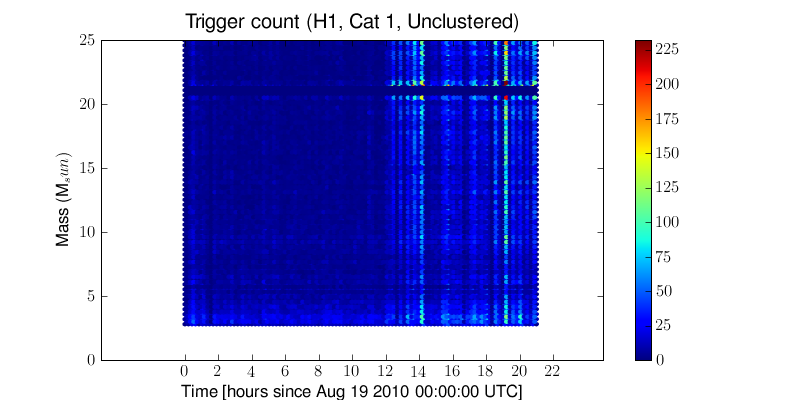
\includegraphics[width=\linewidth]{figures/detchar/H1_1_UNCLUSTERED_hexmass}
  \caption[Trigger rates as a function of time and template length]{
  \label{f:daily_ihope_time_mass}
Trigger rates as a function of time and template length.  The elevated
trigger rate after 12:00 is visible here as well.  Note that
particularly loud glitches, such as that around 19:30, ring off the
entire bank.
}
\end{figure}%


\weakheader{8.  The $\chisq$ test}

These plots showed all triggers with SNR values on the $x$-axis and
$\chisq / (2p-2)$ (the reduced $\chisq$) on the $y$-axis as a way to
visualize the glitchiness of the data.  These plots are most useful
when compared to a reference plot generated from a day of simulated
Gaussian noise, shown in figure \ref{f:gaussian_snr_chisq}, and
comparing the plots at different veto levels, shown in figure
\ref{f:daily_ihope_snr_chisq}.

\begin{figure}
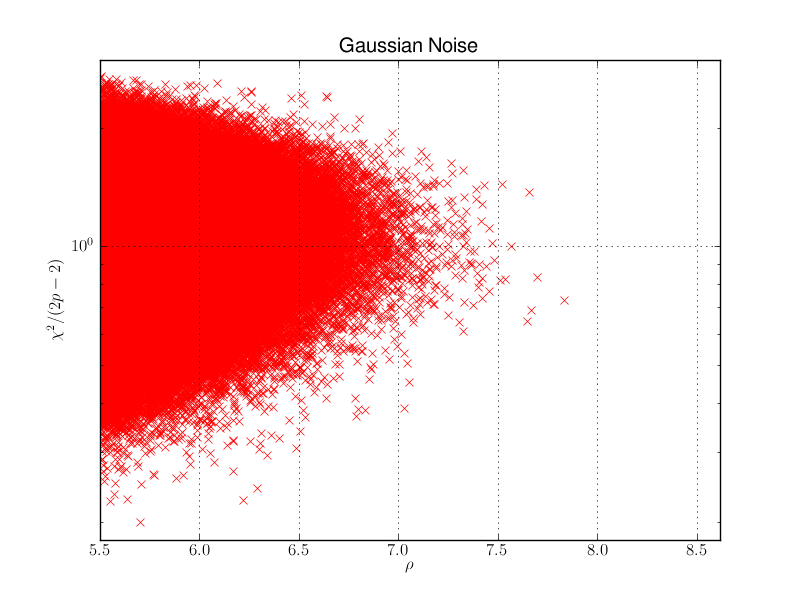
\includegraphics[width=0.85\linewidth]{figures/detchar/GAUSSIAN_0_UNCLUSTERED_chisq.png}
\caption[SNR/reduced $\chisq$ values in Gaussian noise]{
\label{f:gaussian_snr_chisq}
The SNR/reduced $\chisq$ plane for a reference day of
Gaussian noise.  This is the product of a $\chisq$ distribution on the
$y$ axis and a Gaussian distribution on the $x$ axis.}
\end{figure}%

\begin{figure}
  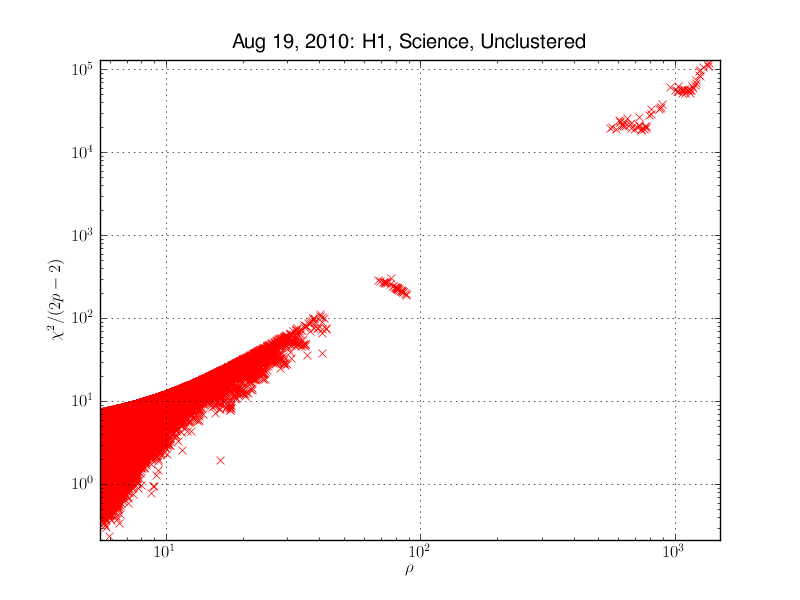
\includegraphics[width=0.5\linewidth]{figures/detchar/H1_0_UNCLUSTERED_chisq.png}
  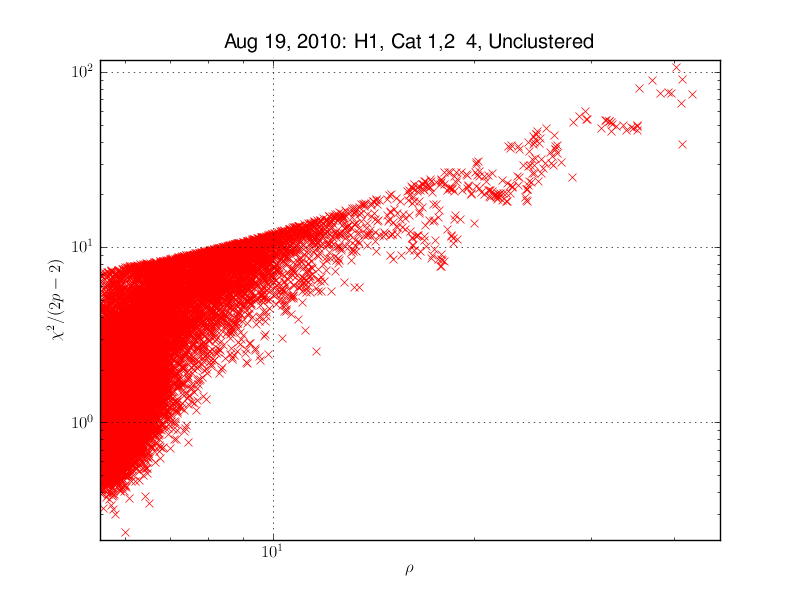
\includegraphics[width=0.5\linewidth]{figures/detchar/H1_4_UNCLUSTERED_chisq.png}
  \caption[SNR/reduced $\chisq$ plots of H1 data.]{
  \label{f:daily_ihope_snr_chisq}
SNR/reduced $\chisq$ plots of H1 data.  The expected shape
of figure \ref{f:gaussian_snr_chisq} is discernible, but there are
long tails of non-Gaussian glitches.  The sharp cutoffs arise 
from thresholds within the inspiral code, see section
\ref{sec:analysis_trigger_selection}.  There is a further
population extending to the upper right at category 0 (left) that is
removed by vetoes in category 4 (right).}
\end{figure}%


\section{Applications of daily ihope to pipeline tuning}
\label{sec:applications_pipeline}

Early in S6 there were frequent instances where the full analysis ran
into difficulty.  This was characterized by individual programs taking
abnormally long to complete, consuming far more than the expected
amount of memory, or failing outright.  The problematic jobs tended to
be individual runs of the \texttt{trigbank} program (see
figure~\ref{f:hipe}); this is the step where triggers from the first
stage are examined to determine which templates need to be used at the
second stage (see figure~\ref{f:hipe}).  Comparing the times that
caused problems to the daily pages immediately revealed a correlation
-- times over which \texttt{trigbank} were unable to run were those
where the rates of triggers were abnormally high.

In S5 and the early weeks of S6 triggers were clustered using a method
called \emph{trigscan}~\cite{SenguptaTrigScan:2008} which attempts to
collapse clusters of triggers that are close in time and parameters to
a single most-significant trigger.  Early versions of the daily page
did this clustering as well, and comparison between the unclustered
and trigscan-clustered triggers revealed that even after clustering
periods of high trigger rates remained~\footnote{Trigscan worked well
in S5, it is not known why it did not work as well in S6.  It is
possible that the instruments were simply more glitchy in the early
days of S6.  However, in order to group triggers together trigscan
must use the bank metric, which was correct in S5 when 2.0 pN
templates were used but incorrect in S6 when the analysis moved to 3.5
pN templates (see section~\ref{sec:bank_metric}).  Some preliminary
investigations were performed, but results were inconclusive}.  This
is illustrated in figure~\ref{f:daily_ihope_high_rates}.  There is a
short period of high trigger rate around 05:40 which remained high
after clustering.  A run of \texttt{trigbank} processing this time was
unable to complete.

The possibility of vetoing such glitchy periods was raised, and this
could have been easy to accomplished using the rate information from
daily ihope.  However, such vetoes would have needed to be category 1 to
avoid the problem, which would mean subdividing science segments and
possibly losing short segments.  Instead we replaced trigscan with
fixed 30-millisecond clustering windows, after studies of found/missed
injections determined that this change did not harm the search
efficiency. 

\begin{figure}
  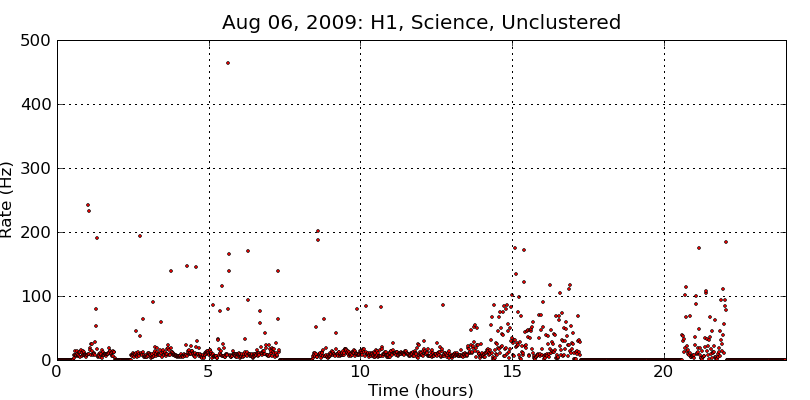
\includegraphics[width=0.5\linewidth]{figures/detchar/20090806_H1_0_UNCLUSTERED_rate_vs_time}
  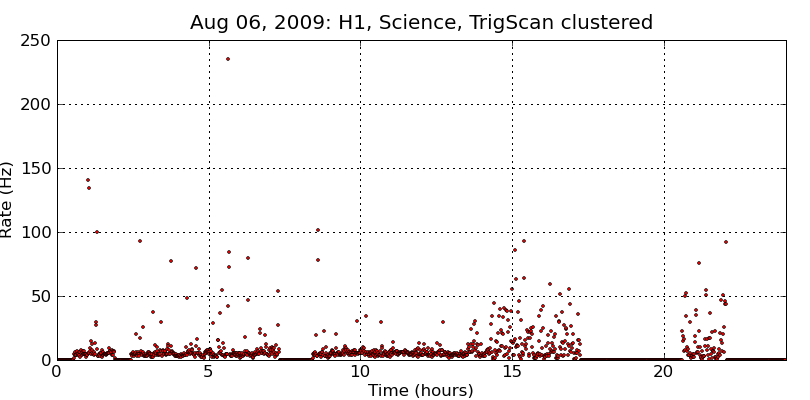
\includegraphics[width=0.5\linewidth]{figures/detchar/20090806_H1_0_TS_CLUSTERED_rate_vs_time}
  \caption[Problematic times identified by daily ihope]{
  \label{f:daily_ihope_high_rates}
Problematic times identified by daily ihope.  The plot on the left
shows the rate of triggers over the day without any clustering.  Note
the sudden jump in rate at 5:40.  On the right, the same plot after
clustering triggers with the trigscan algorithm.  The overall rate has
been reduced by about a factor of two, indicated by the different
scales on the y axes.  However, the rate remains high enough to cause
problems.
}
\end{figure}%

At the start of S6 the range of the low-mass search extended up to $35
\msun$, as it did in S5.  However, along with times of high trigger
rates, the daily ihope pages indicated that most of the triggers were
coming from the high-mass end of the bank.  This behavior is expected,
as it is easier for short templates to match against glitches, but the
trigger histograms highlighted the extent to which this was a problem.
A sample plot of triggers per template from early S6 is shown on the
left of figure~\ref{f:daily_ihope_el_glitcho}.  It shows that the
shortest template in the bank, with $m_1 = m_2 = 17.5 \msun$ was
producing significantly more triggers than any other template.  In
part this was due to a bug in the template bank code, that caused this
template to appear twice in some banks.  In part the abundance of
triggers from this template is due to it appearing in every bank
throughout the day, whereas other templates tend to get repositioned
as the noise curve changes.  Even taking these effects into account,
most of the triggers come from templates shorter than 5 seconds, as
seen on the right of figure~\ref{f:daily_ihope_el_glitcho}.

The fixed clustering window means that only the loudest trigger in a
30-millisecond window will be passed to subsequent stages of the
analysis.  Given the numbers of triggers from short templates there
was concern that a loud, short glitch could mask a quieter trigger
from a binary neutron star coalescence.  We therefore decided to limit
the low-mass search to $M < 25 \msun$ after comparing found/missed
plots of injections in the same weeks with the different mass ranges,
and determining that the smaller bank did as well or better than the
larger bank.


\begin{figure}
  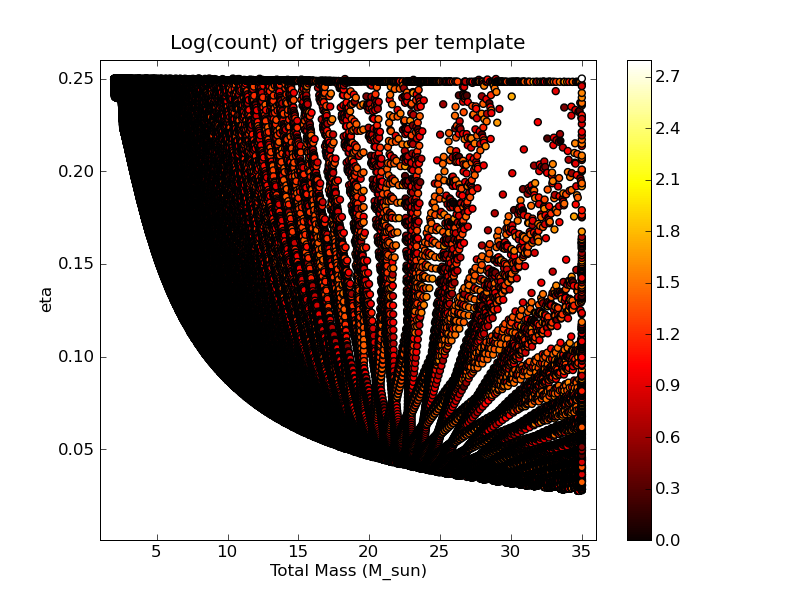
\includegraphics[width=0.5\linewidth]{figures/detchar/20090806_H1_0_UNCLUSTERED_template_counts}
  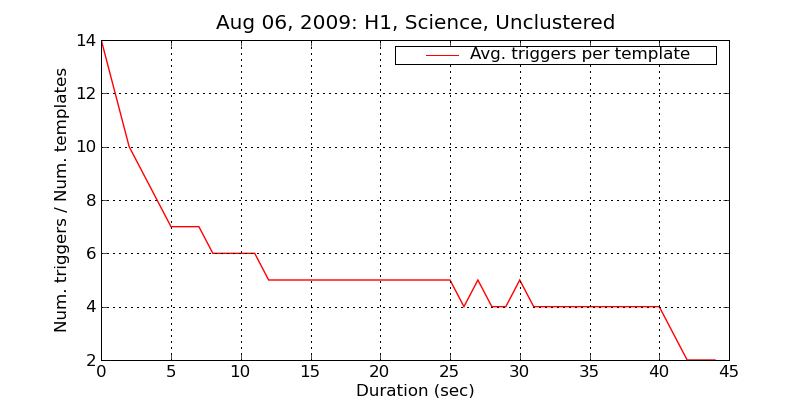
\includegraphics[width=0.5\linewidth]{figures/detchar/20090806_H1_0_UNCLUSTERED_mass_hist_norm}
  \caption[Problematic templates seen in daily ihope]{
  \label{f:daily_ihope_el_glitcho}
Problematic templates seen in daily ihope.  This shows the equivalent
of figures~\ref{f:daily_ihope_time_mass} and
\ref{f:count_per_template} from an earlier version of daily ihope and
an earlier version of the CBC search.  Note the excess of triggers
from the high-mass end of the bank, corresponding to shorter
templates.
}
\end{figure}%



\section{Applications of daily ihope to individual vetoes}
\label{sec:applications_vetoes}


The categories used by daily ihope differ slightly from those
used by the full analysis.

Category 1 vetoes indicates time that should not have been marked as
science mode.  Typically attempting to analyze this time will
adversely affect the entire 2048-second analysis chunk, for example by
biasing the PSD (section \ref{sec:ihope_psd}).  Note that it is
possible to correct science time by creating a new version of the
\texttt{DMT\_SCIENCE} flag with an incremental version number.
However, doing so is a more complicated process than creating a veto
flag, and removing time by denoting it CAT1 carries additional
information about the reason for the veto.  Note that category 1
vetoes are undesirable, as they may remove time outside the range of
the problem.  For example, a 4080-second span of science-mode data
with a one-second CAT1 veto at 2040 seconds will be completely
unanalyzable by the CBC group, as excising the bad data will leave no
contiguous 2048-second block.

Category 2 vetoes indicates time during which there was a problem,
instrumental or environmental, with well-understood coupling into
\texttt{DARM\_ERR}.  Such time can be analyzed without problem, but
triggers from such time will be discarded. 

Category 3 vetoes remove hardware injections (section
\ref{sec:ihope_hardware_injections}).  In the full analysis hardware
injection vetoes do not have a category number and is denoted
``hardware injections removed.''

Category 4 is for time that appears to be ill-behaved according to 
data quality studies, but where there is no clearly-understood 
cause.  In the full analysis this is denoted category 3.
In addition to tracking the performance of the pipeline as a whole,
daily ihope was used to flag numerous glitch mechanisms throughout the
course of S6.  Such glitches typically showed up in the rate vs. time
plot, the SNR vs. time plot, and/or the list of loudest triggers.
Often these were spotted either by individuals reviewing the pages on
a daily basis, by an individual in the CBC group assigned  to do
glitch studies preceding a run of the full analysis pipeline, or by
the group during reviews of these studies.

As patterns emerged from these results members of the detector
characterization group would work with the commissioners to identify
the underlying causes, and simultaneously work with data analysts to
develop and test vetoes.  Often these vetoes were verified by running
a script, \texttt{lalapps\_check\_flag} which, given a file
containing veto segments and a time range would report on the
efficiency and deadtime of the veto by applying it to the daily ihope
triggers over the specified time range.  The file could be generated
from an existing flag in the database using {\texttt
ligolw\_dq\_query} (see chapter~\ref{ch:segdb}), or it could be
generated by a script looking at auxiliary channel information
provided by Omega or klinewelle triggers.

We now give examples of the use of daily ihope in constructing vetoes
at each level.

\subsection{Category 1}

\weakheader{Glitches from the Thermal Compensation System}

The design of the LIGO mirrors accounted for the fact that in
operation they would be heated by the laser and the radius of
curvature would change.  However, in S6 as we moved to higher laser
power the mirror's absorption of energy was larger than expected and
the mirror overheated and deformed more than expected~\cite{}.  To
correct for this a compensating laser was added that would heat the
mirror in a ring in order to restore the radius of curvature to an
optimal value.  However, this laser would occasionally glitch, kicking
the mirror and producing loud noise in the detector.

The identification of these glitches was straightforward; they were
often the loudest glitches of the day and were readily visible in the
daily ihope ``loudest trigger'' report, as well as similar reports
generated by KW and Omega.  The cause was similarly easy to identify,
as the omega scans generated by daily ihope showed egregious behavior
in the TCS channels.  An automated veto based on a threshold value in
the TCS channel was added to the DMT at category 2.  However, some
instances were loud enough to interfere with the CBC pipeline in
surrounding times, hence it was decided to veto these times at
category 1.  These features are illustrated in
figure~\ref{f:daily_ihope_tcs}.  


%
% P. Willems, "Thermal Compensation in the LIGO Gravitational-Wave
% Interferometers," in Adaptive Optics: Methods, Analysis and
% Applications, OSA Technical Digest (CD) (Optical Society of America,
% 2009), paper AOThA5.
% http://www.opticsinfobase.org/abstract.cfm?URI=AO-2009-AOThA5
% 

\begin{figure}
  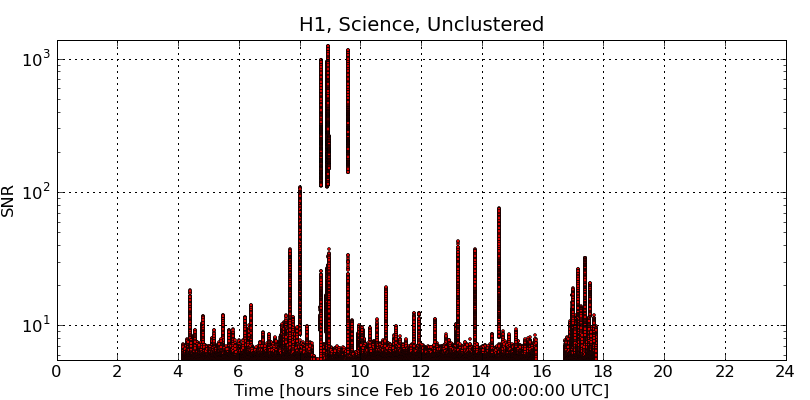
\includegraphics[width=0.5\linewidth]{figures/detchar/20100217_H1_0_UNCLUSTERED_snr_vs_time} 
  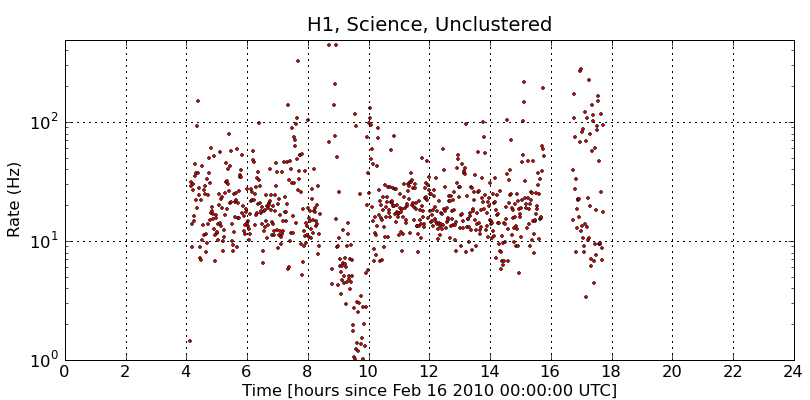
\includegraphics[width=0.5\linewidth]{figures/detchar/20100217_H1_0_UNCLUSTERED_rate_vs_time} \\
  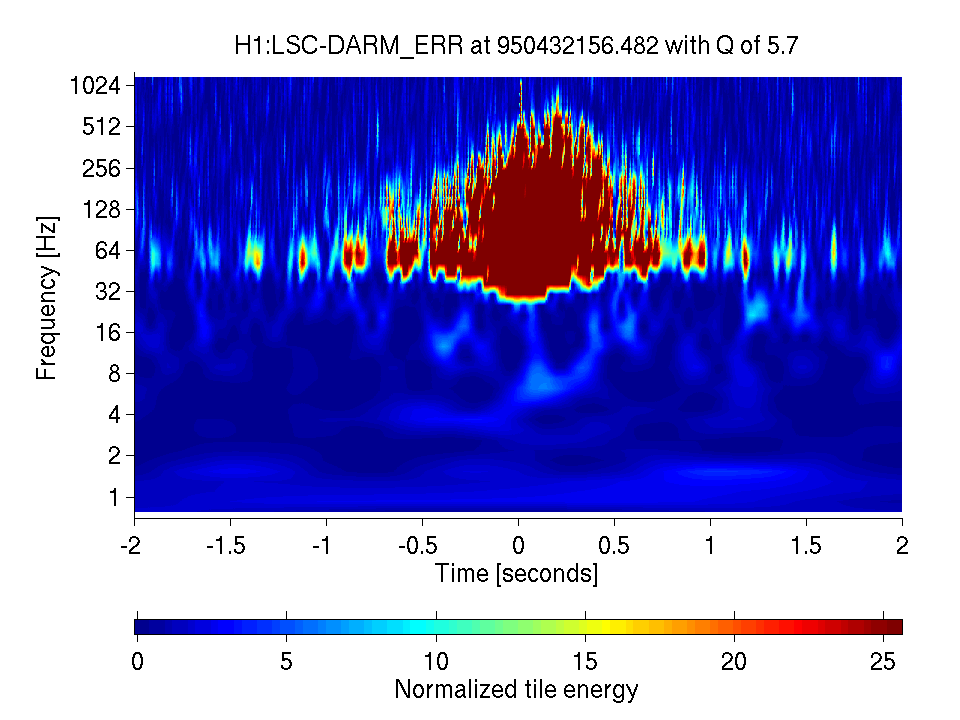
\includegraphics[width=0.5\linewidth]{figures/detchar/950432156_482177734_H1_LSC-DARM_ERR_4_00_spectrogram_whitened}
  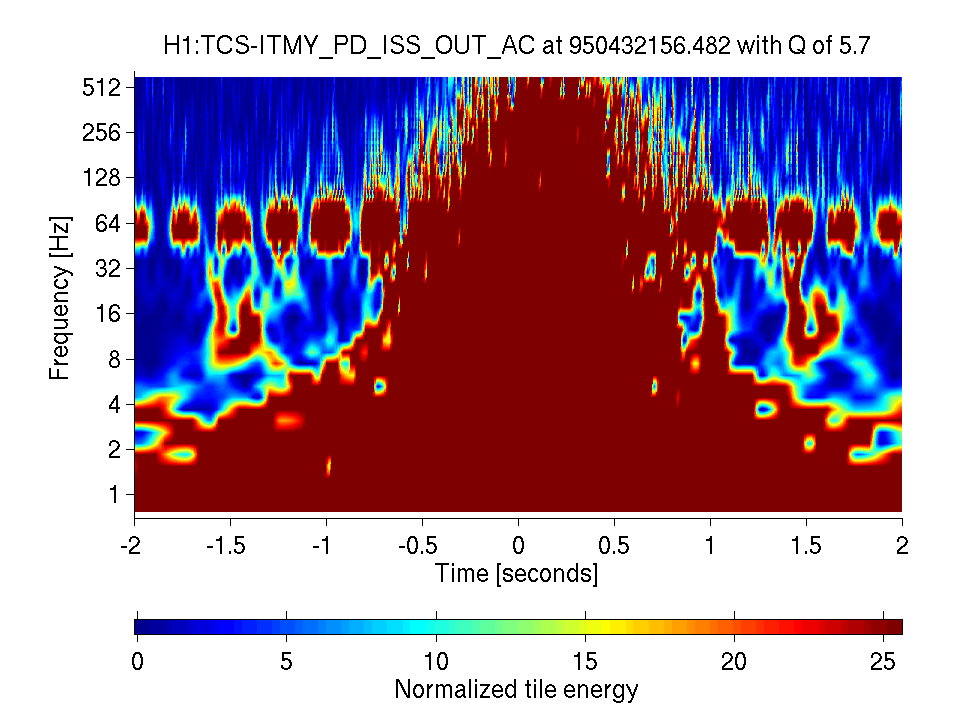
\includegraphics[width=0.5\linewidth]{figures/detchar/950432156_482177734_H1_TCS-ITMY_PD_ISS_OUT_AC_4_00_spectrogram_whitened}
  \caption[TCS glitch in daily ihope and omega]{
  \label{f:daily_ihope_tcs}
TCS glitches in daily ihope and followup omega scans.  The top left
shows the SNR as a function of time, the loudest triggers are all TCS
glitches.  Note that each loud glitch comes in the form of a ``tower''
containing many triggers.  This phenomena will be discussed further in
section~\ref{ssec:penguins}.  This is further illustrated by the trigger
rate plot (top right), which shows elevated trigger rates at the times
of the glitch.  Note that around the time of the glitch the trigger
rate actually {\it drops} significantly.  This will be discussed in
section~\ref{ssec:sarlacc}, but indicates that the glitches are loud
enough to interfere with the analysis in surrounding times, justifying
the use of a CAT 1 veto.  The lower left plot shows the omega scan
of the gravitational-wave output channel at the time of the loudest
glitch, clearly showing that this is not a gravitational wave.  The
lower right plot shows the omega scan of a channel monitoring the TCS,
identifying it as the source of the glitch.}
\end{figure}%


\weakheader{Grid glitches}

This was a loud, broad-band glitch that produced a grid of triggers in
the KW pipeline's time-frequency plane, where the phenomena was first
seen.  They also showed up in the daily ihope rate and SNR plots as
loud triggers accompanied by elevated trigger rates, as shown in
figure~\ref{f:omega_grid}.  These also often appeared on the
daily list of loudest glitches, the omega scans generated by daily
ihope showed problems in magnetometers and the output mode cleaner
photodiodes, this is shown in figure~\ref{f:omega_grid}.  As with the
TCS glitches, instances that showed up particularly loudly in daily
ihope were hand-vetoed at category 1.  The problem was eventually
traced to a power supply, once this was resoldered the problem
disappeared.

% https://wiki.ligo.org/foswiki/bin/view/DetChar/CurrentUnvetoedGlitchClasses
% https://wiki.ligo.org/DetChar/H1GridGlitchStory

% Example: 
% tconvert 963852915
% Jul 22 2010 16:55:00 UTC

\begin{figure}
  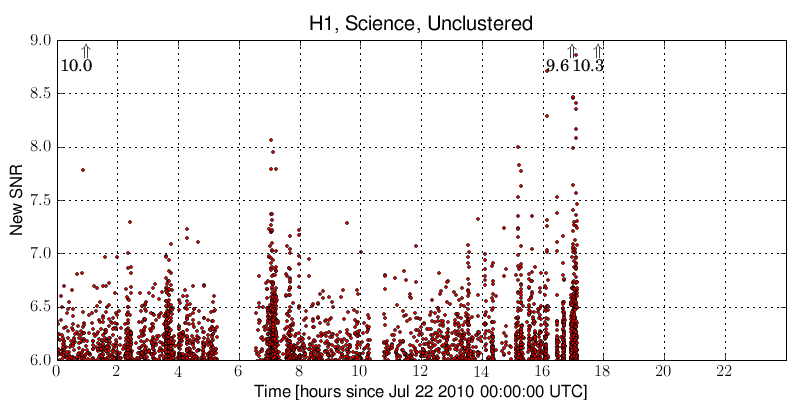
\includegraphics[width=0.5\linewidth]{figures/detchar/20100722_H1_0_UNCLUSTERED_newsnr_vs_time}
  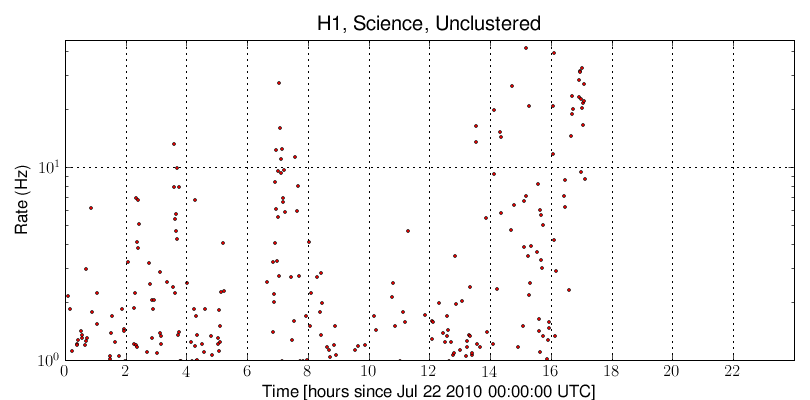
\includegraphics[width=0.5\linewidth]{figures/detchar/20100722_H1_0_UNCLUSTERED_rate_vs_time}
  \caption[Grid glitches in daily ihope] {
  \label{f:daily_ihope_grid}
Grid glitches as seen by daily ihope.  The plot on the left shows
$\newsnr$, with the grid glitches indicated by arrows pointing above
the range at which the plot cuts off (auto-scaling of this plot was
removed from daily ihope to prevent a single loud glitch from
squeezing all the other data to a thin region at the bottom of the
plot).  Note that the high value indicates that this glitch is fooling 
the $\chisq$ signal-based veto.  The plot on the right shows the
associated increase in trigger rate.
}
\end{figure}%

\begin{figure}
  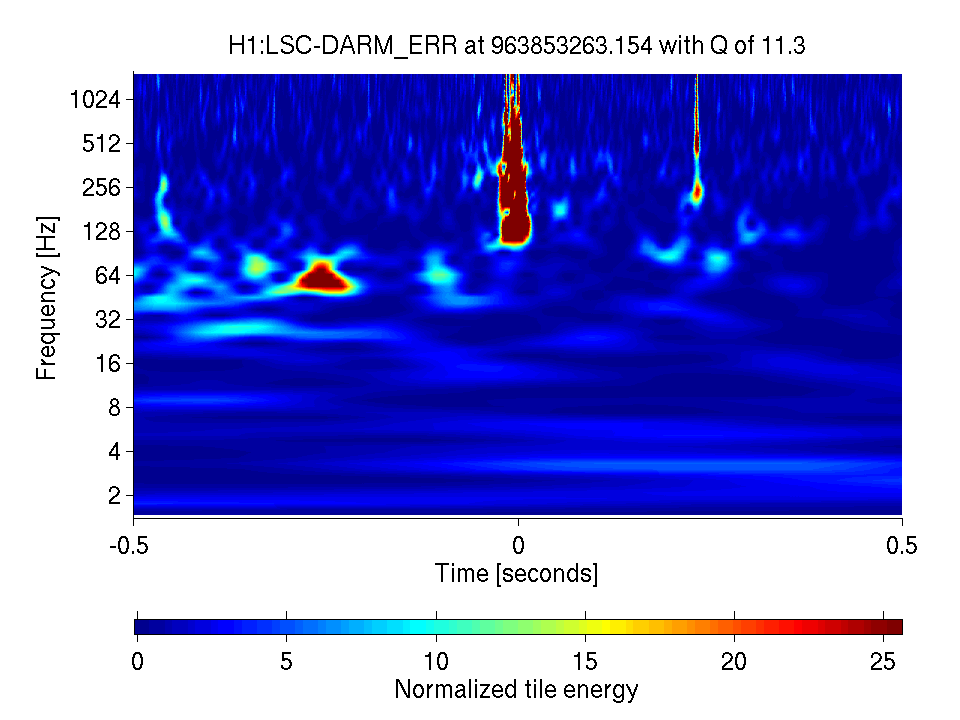
\includegraphics[width=\linewidth]{figures/detchar/963853263_154296875_H1_LSC-DARM_ERR_1_00_spectrogram_whitened}
  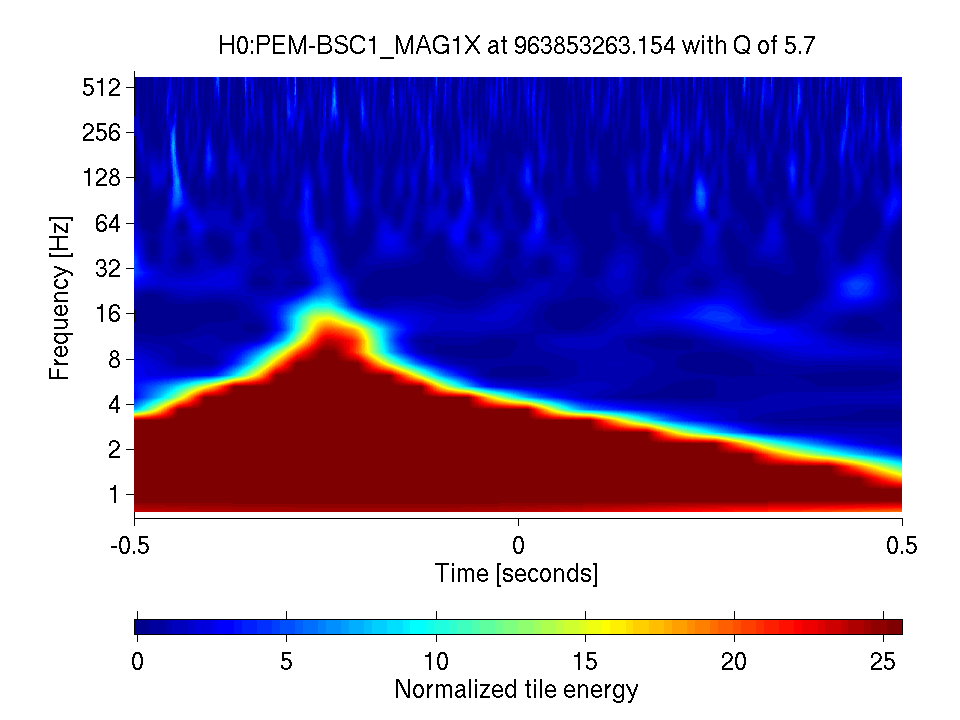
\includegraphics[width=0.5\linewidth]{figures/detchar/963853263_154296875_H0_PEM-BSC1_MAG1X_1_00_spectrogram_whitened}
  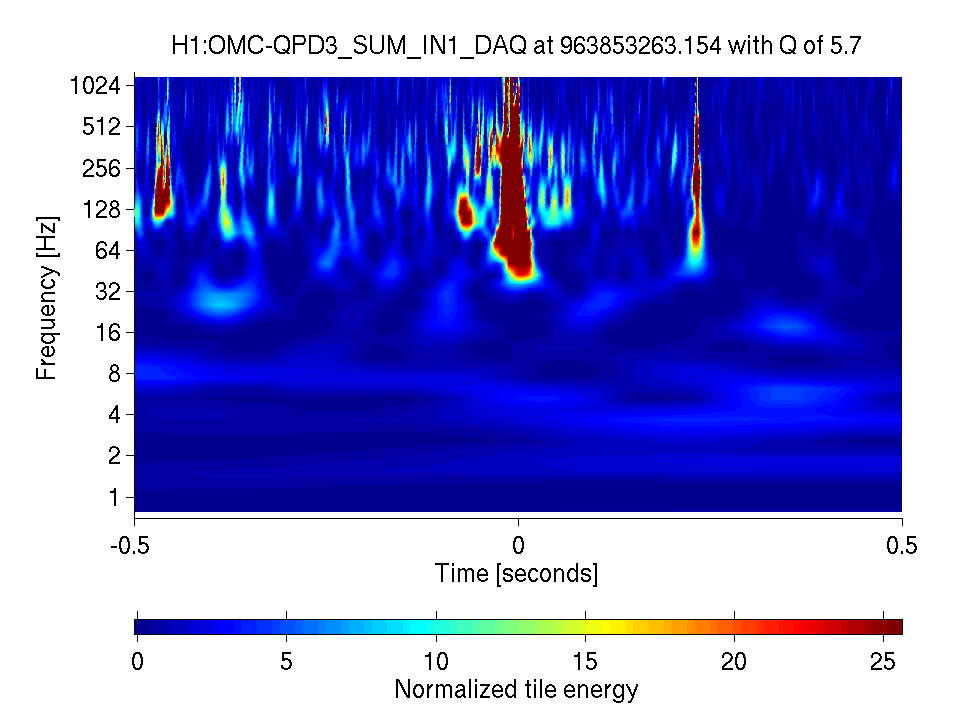
\includegraphics[width=0.5\linewidth]{figures/detchar/963853263_154296875_H1_OMC-QPD3_SUM_IN1_DAQ_1_00_spectrogram_whitened}
  \caption[Grid glitches in omega]{
  \label{f:omega_grid}
Omega scans of the grid glitch flagged as the loudest trigger of the
day and visible as an arrow in figure~\ref{f:daily_ihope_grid}.  At
the top, the gravitational-wave output channel, and at the bottom two
channels that were associated with this class of glitch.
}
\end{figure}%


\subsection{Category 2}

\weakheader{The spike glitch}

The spike glitch was a very loud, very short ``bang'' in the
Livingston detector, characterized by a sudden drop in \darmerr
immediately followed by a sharp increase.  An example is shown in
figure~\ref{f:spike_glitch_example}.  In some cases there were a few
cycles of ringing before the channel settled back down.  These often
produced SNR values of several thousand.  The $\chisq$ values were
typically large for the events themselves, resulting in negligible
$\newsnr$ values.  However, the triggers in the tails (see
section~\ref{ssec:penguins}) could have large new SNR values.  A
sample daily ihope plot with several spike glitches and representative
omega scans are shown in figure~\ref{f:daily_spikes}.

\begin{figure}
  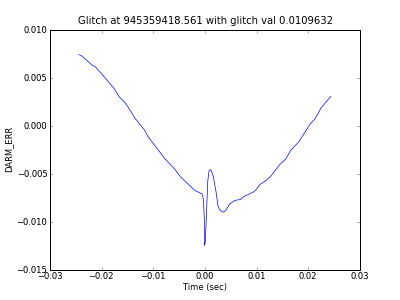
\includegraphics[width=\linewidth]{figures/detchar/spike_glitch_example}
  \caption[The spike glitch]{
  \label{f:spike_glitch_example}
A sample spike glitches in \darmerr.  Note the characteristic
down-up-down pattern, and short timespan.}
\end{figure}%

Despite a great deal of effort by lots of people, the cause of these
glitches was never identified.  However, the distinctive shape allowed
the creation of an automated veto.  \texttt{LSC\_STRAIN} was sampled
every half-millisecond, giving a time series $x_i$.  For each sample
$i$ the quantity 

\begin{equation*}
x_i - 2 x_{i+1} + x_{i+2} 
\end{equation*}

was calculated, values exceeding a threshold indicated a possible
spike and the time was flagged in the segment database.  Not every
time so-flagged was a spike, but every instance indicated a
potentially problematic rapid fluctuation in the data.



% https://wiki.ligo.org/foswiki/bin/view/DetChar/S6L1OMCGlitchVeto

% DCH-SPIKE_GLITCH (0,4)

% Example 947204646.611816406
% Jan 11 2010 00:23:51.611816406 UTC == SNR 8849


\begin{figure}
  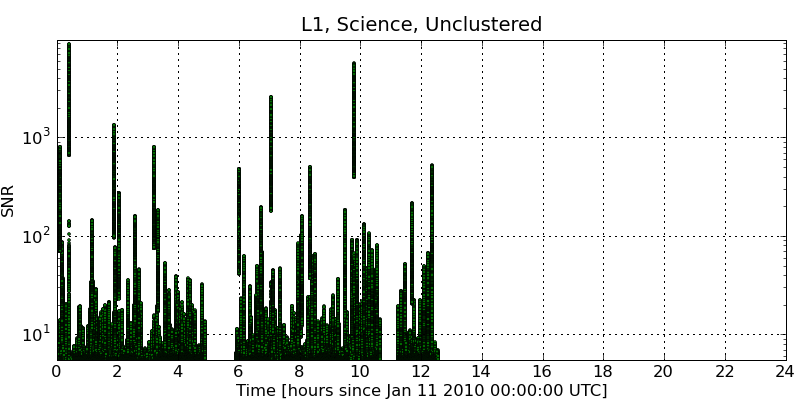
\includegraphics[width=\linewidth]{figures/detchar/20100111_L1_0_UNCLUSTERED_snr_vs_time} \\
  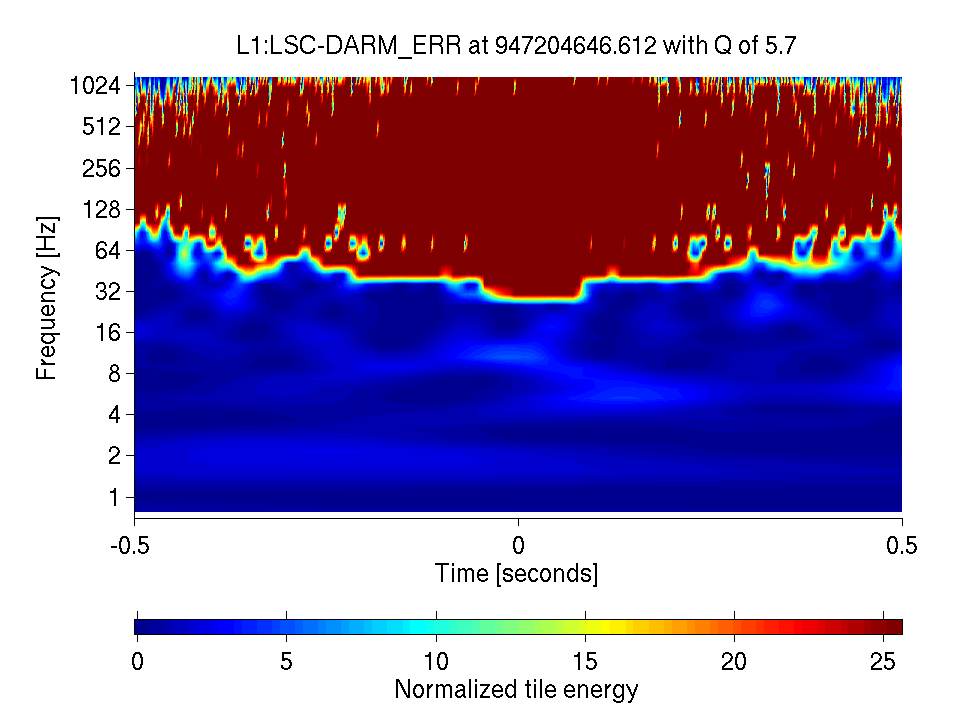
\includegraphics[width=0.5\linewidth]{figures/detchar/947204646_611816406_L1_LSC-DARM_ERR_1_00_spectrogram_whitened}
  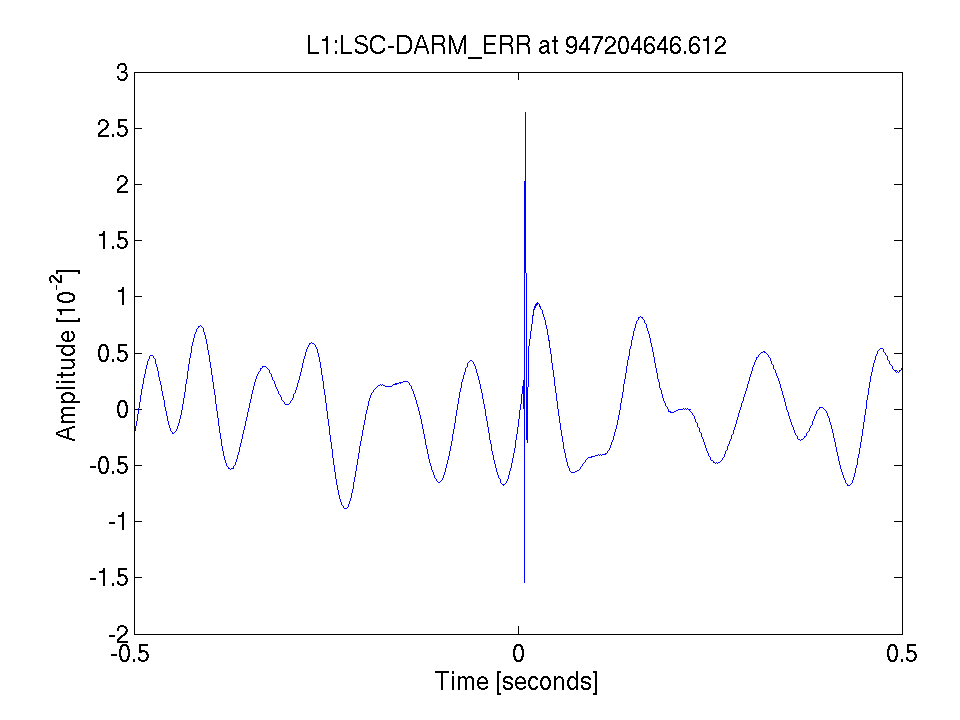
\includegraphics[width=0.5\linewidth]{figures/detchar/947204646_611816406_L1_LSC-DARM_ERR_1_00_timeseries_raw}
  \caption[Spike glitch in daily ihope and omega]{
  \label{f:daily_spikes}
  Spike glitches in daily ihope and a typical omega scan.  At the top
a daily ihope SNR-vs-time plot, showing several spike glitches with
SNRs of several thousand.  On the bottom, the loudest of these spike
glitches in an omega scan, showing the time-frequency plot (left) and
unfiltered time series (right).  The sharp drop-rise-drop of the time
series behavior was reasonable well-captured by the filtered used to
create data quality segments.
}
\end{figure}%

\weakheader{HEPI glitches}

Livingston is subject to seismic activity, both natural and
anthropogenic, that does not effect the Hanford detector.  In order
for the L1 detector to achieve the same low-frequency response it is
therefore necessary to take additional steps.  The Hydraulic External
Pre-Isolation (\emph{HEPI}) system sits between the ground and
chambers containing optical components and provides a layer of active
seismic isolation.  This can reduce noise in the 1-3 Hz band by a few
percent~\cite{Wen:thesis}.

In early 2010 it was noticed that the daily ihope triggers contained
several instances with SNRs above 600 even after applying all known
vetoes through category 4.  This included removal of spike glitches
and application of the use-percentage vetoes (discussed in the next
section).  Followup of these triggers in the daily loudest-glitch
reports showed that they were all accompanied by loud glitches in the
HEPI channels.  Samples are shown in figure~\ref{f:daily_hepi}.

A trial veto was created by scanning the auxiliary channel time series
for values exceeding 25,000.  This veto was tested by applying it to
the remaining daily ihope triggers, and it was found to be very
effective.  Histograms of triggers before and after application of
this veto are shown in figure~\ref{f:hepi_veto_effectiveness}.  After
this confirmation the veto was applied at category 2 to the full
search.

A great deal of work was done on HEPI during this period, and after
Jan 10, 2010 the problem ceased.

% DCH-SEI_ITMY_Y_OVER_25000
% example 946834715.499755859 == Jan 06 2010 17:38:20 UTC
% https://ldas-jobs.ligo.caltech.edu/~cbc/ihope_daily/201001/20100106/
% 5th loudest in day
%
% https://wiki.ligo.org/foswiki/bin/view/DetChar/CBC_S6B_L1_SingleDetectorLoudest
% After applying CAT 2, 3, and 4, including UPV and the Spike glitch
% veto, there are still many loud triggers in the CBC single-detector
% background. This does not include the effect of chi squared or
% coincidence. The triggers above SNR 600 are: 
%
% https://ldas-jobs.ligo.caltech.edu/~lundgren/DataQuality/Issues/HEPI/L1-S6B2-snrhist_Cat1234_Spike_HEPI.png
%
% http://www.ligo.caltech.edu/LIGO_web/0409news/0409liv.html


\begin{figure}
  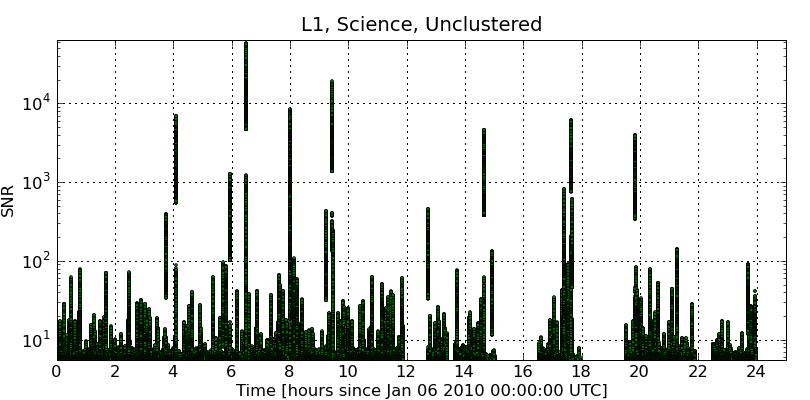
\includegraphics[width=0.5\linewidth]{figures/detchar/20100106_L1_0_UNCLUSTERED_snr_vs_time}
  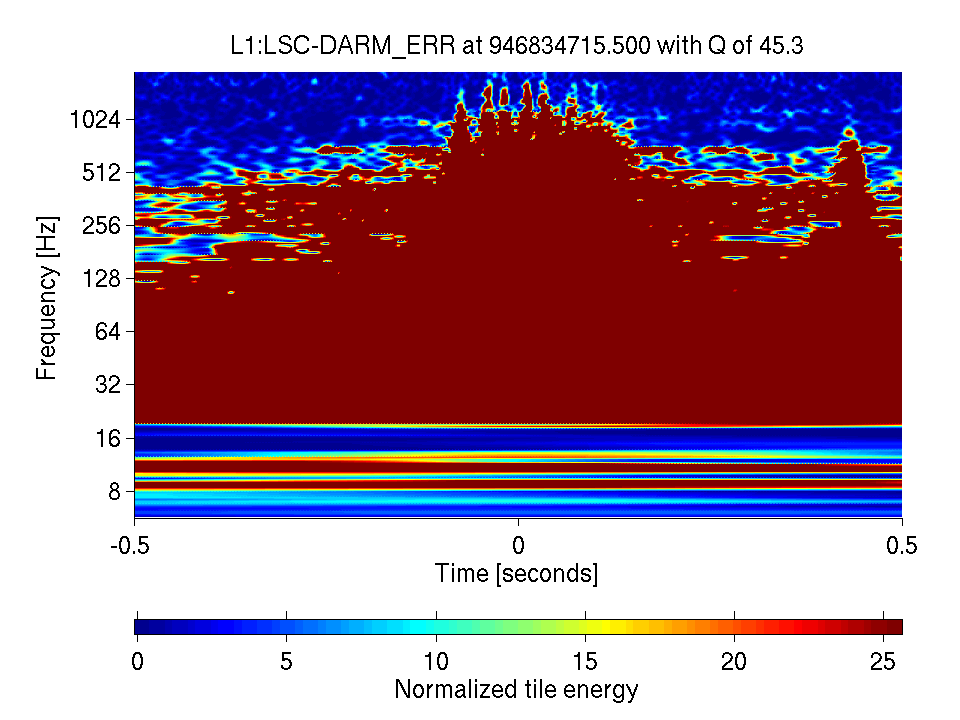
\includegraphics[width=0.5\linewidth]{figures/detchar/946834715_499755859_L1_LSC-DARM_ERR_1_00_spectrogram_whitened} \\
  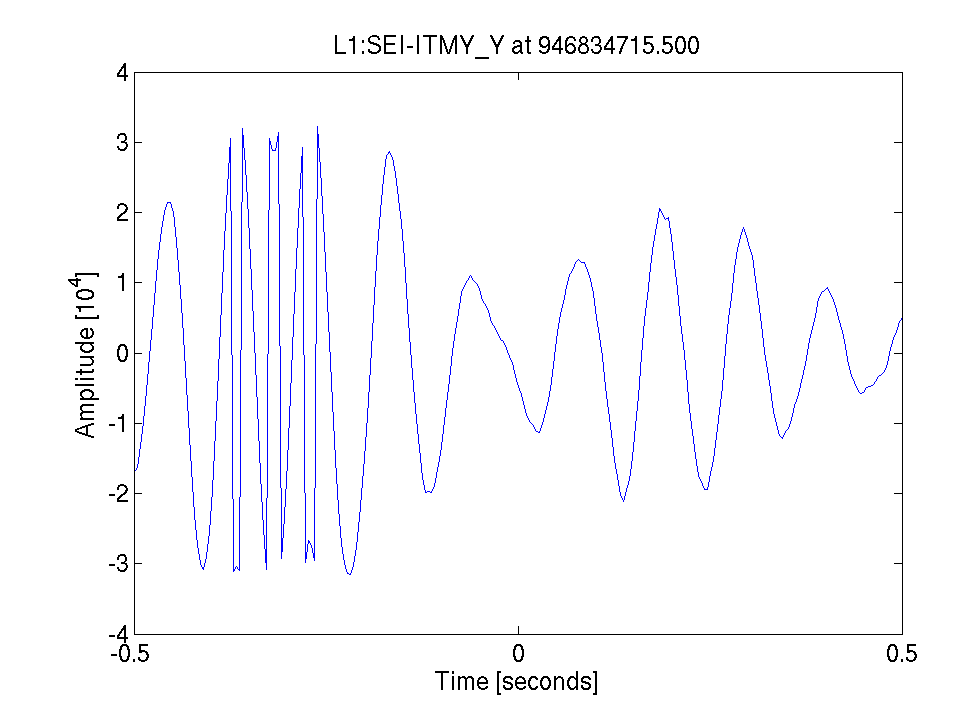
\includegraphics[width=0.5\linewidth]{figures/detchar/946834715_499755859_L1_SEI-ITMY_Y_1_00_timeseries_raw}
  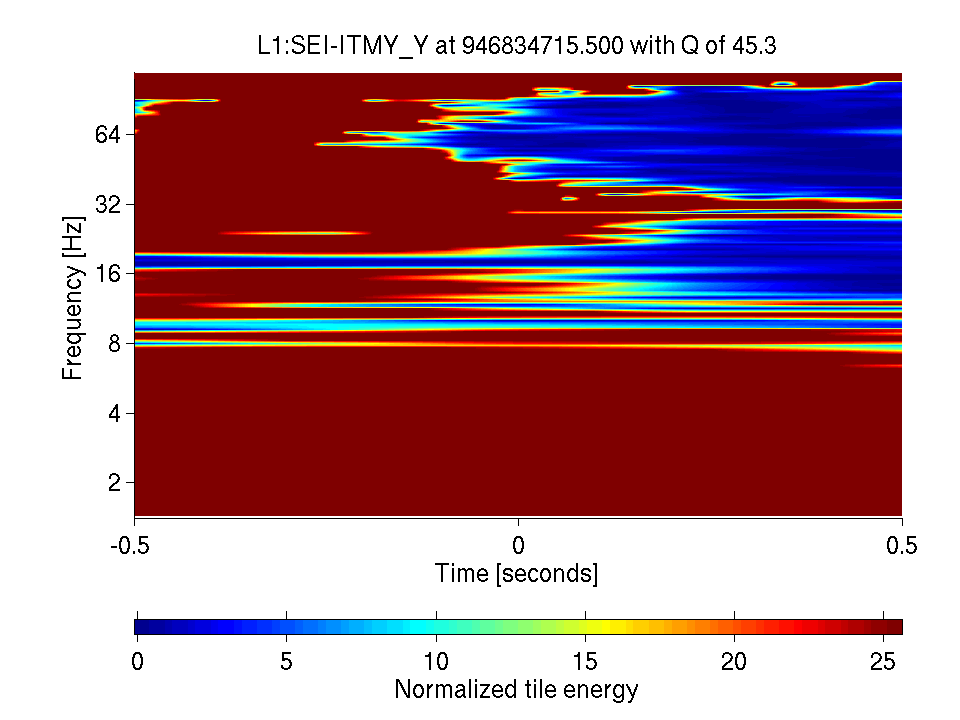
\includegraphics[width=0.5\linewidth]{figures/detchar/946834715_499755859_L1_SEI-ITMY_Y_1_00_spectrogram_whitened}
  \caption[The HEPI glitch in daily ihope and Omega]{
  \label{f:daily_hepi}
The HEPI glitch in daily ihope and Omega.  On the top left, the SNR
values for the day including a HEPI glitch at 17:38, as identified by
the ``loudest glitches'' report.  On the top right, this event in
\darmerr.  On the bottom left the time-frequency plot of a HEPI
auxiliary channel, and on the bottom right the unfiltered time series
of this same channel, showing that it has exceeded the threshold of
25,000}
\end{figure}%

\begin{figure}
  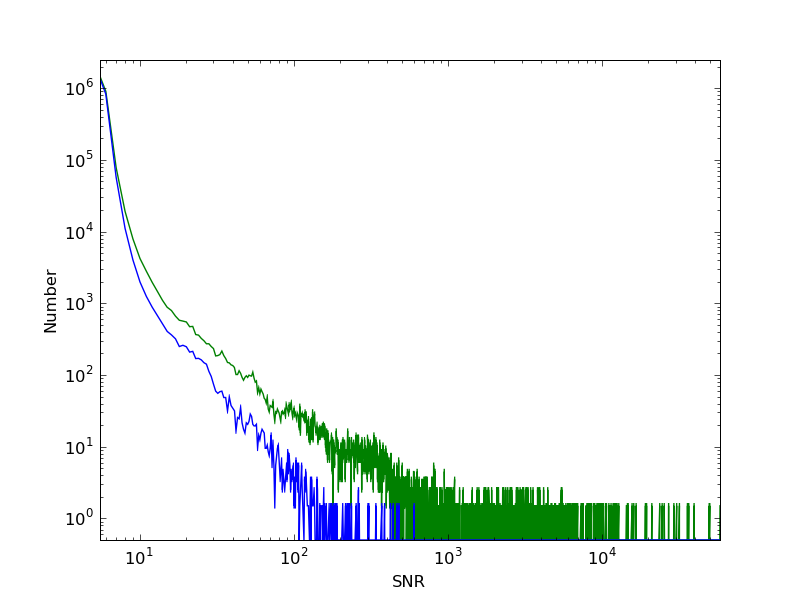
\includegraphics[width=\linewidth]{figures/detchar/L1-S6B2-snrhist_Cat1234_Spike_HEPI}
  \caption[Effectiveness of the HEPI veto] {
  \label{f:hepi_veto_effectiveness}
Effectiveness of the HEPI veto. The green line shows the number of
daily triggers after applying all known vetoes, including the removal
of spike glitches.  The blue line show counts after the additional
HEPI veto is applied.  Note that the highest SNR is reduced from 
4,000 to 600, along with a reduction of triggers at SNRs down to 
$~ 10$.}
\end{figure}


\subsection{Category 4}

% https://wiki.ligo.org/foswiki/bin/view/DetChar/H1LVEASEISZS6Cflag

\weakheader{Automated vetoes}

There were three uses of the daily triggers through S6.  The first
two, the daily pages and ad-hoc veto studies, have already been
discussed.  The third was as input to systematic automated veto
studies.

\emph{SeisVeto}~\cite{} compared low-frequency triggers from Omega
running on seismic PEM channels to daily ihope triggers using the
\emph{HVeto}~\cite{} algorithm.  Times of high correlation were
flagged with category 4 vetoes, which could achieve up to 62\%
efficiency with only 6\% deadtime.

The \emph{Used Percentage Veto} (UPV) program looked for correlations
between triggers from \darmerr and auxiliary channels using a figure
of merit defined as

\begin{equation*}
\textrm{Used Percentage}(\rho) \equiv 100 \times
N_\textrm{coinc}(\rho) / N_\textrm{total}(\rho)
\end{equation*}

where $N_\textrm{total}(\rho)$ is the total number of triggers from
the auxiliary channel above significance threshold $\rho$ in the
analysis time, and $N_\textrm{coinc}(\rho)$ is the number of trigger
from the auxiliary channel that lie within a second of a trigger from
\darmerr.  Intervals where this percentage exceeded 50\% were entered
into the segment database and applied as category 4 vetoes.  Although
UPV was originally developed using KW triggers for both \darmerr and
auxiliary channels, it was modified during S6 to accept triggers from
daily ihope.  The resulting analysis was rerun weekly.


% UPV-IHOPE_H1_ASC_WFS2_IY_8_256_100 (in C) and more
% (tconvert 957191412, May 06 2010 14:29:57 UTC)
% Accompanied by rate > 500 Hz (=866) for 4 seconds, slight elevation in SNR

An example is shown in figure~\ref{f:daily_upv}.  During the week
including this day UPV determined that the instrumental channel
\texttt{ASC-WFS2\_IY} \Note{brief description} had a high correlation
with daily triggers.  This is a quiet glitch, with an SNR of 6.5, and
it would have taken considerable effort to track down manually.
However, it is accompanied by 4 seconds of elevated trigger rates
which could have impacted the search and should therefore be flagged
at category 4.

\begin{figure}
  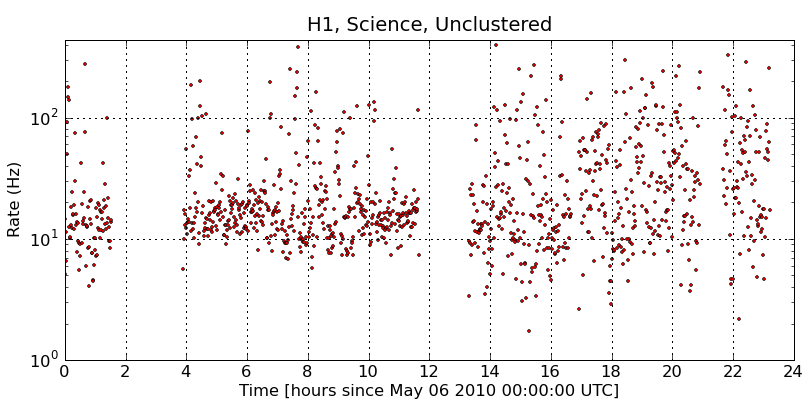
\includegraphics[width=0.5\linewidth]{figures/detchar/20100506_H1_0_UNCLUSTERED_rate_vs_time}
  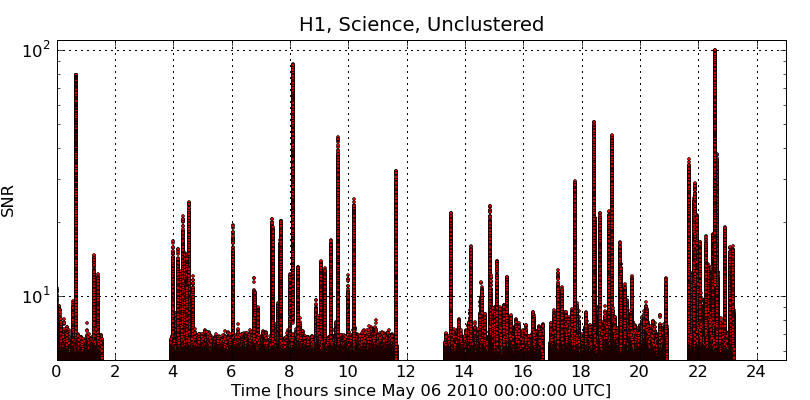
\includegraphics[width=0.5\linewidth]{figures/detchar/20100506_H1_0_UNCLUSTERED_snr_vs_time} \\
  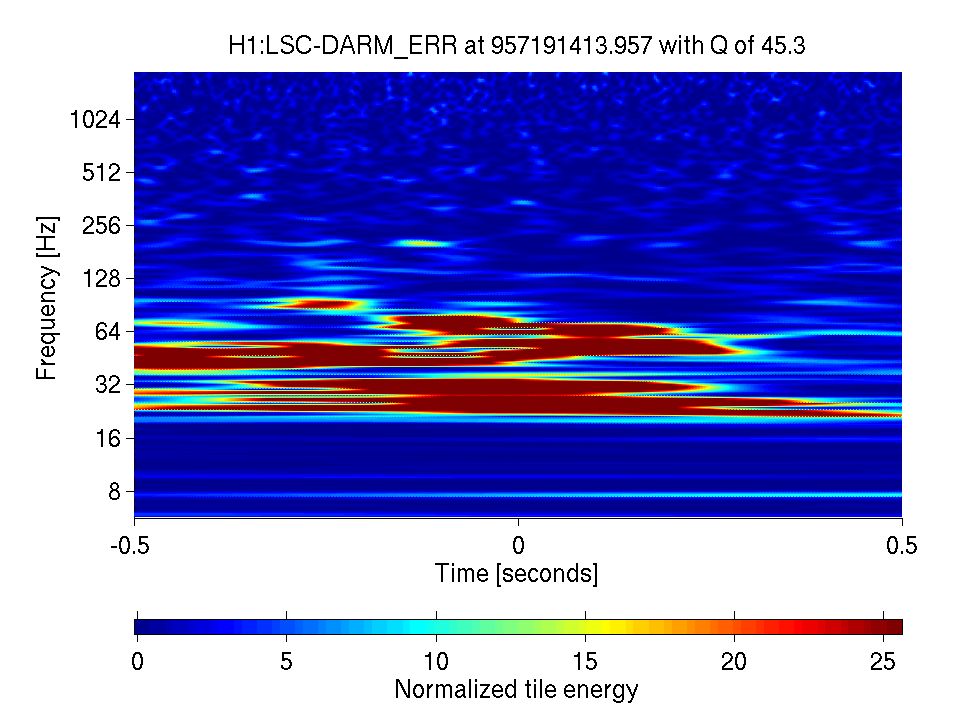
\includegraphics[width=0.5\linewidth]{figures/detchar/957191413_957191417_H1_LSC-DARM_ERR_1_00_spectrogram_whitened}
  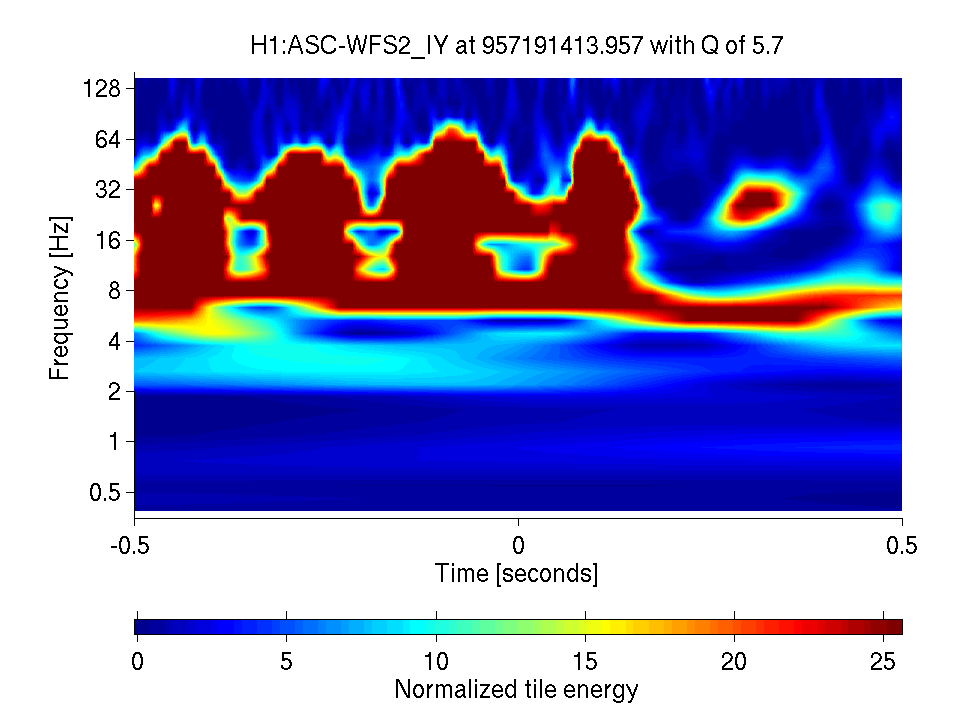
\includegraphics[width=0.5\linewidth]{figures/detchar/957191413_957191417_H1_ASC-WFS2_IY_1_00_spectrogram_whitened}
  \caption[Glitch found by UPV using the daily triggers]{
  \label{f:daily_upv}
A glitch found by UPV using the daily triggers.  On the top the daily
rate and SNR plots, including the glitch in question at 14:29.  On the
bottom the omega scan of \darmerr and the auxiliary channel whose KW
triggers correlate with daily ihope darmerr triggers.}
\end{figure}%

\weakheader{Loud SNR}

Through the S6 run the \emph{horizon distance}, the distance at which
the coalescence of an optimally-oriented binary system consisting of
two $1.4 \msun$ neutron stars would have an SNR of 8, was roughly 30
Mpc.  The SNR scales inversely with distance, hence the distance at
which we would expect to see such a system at, say, SNR 250 is 0.12
Mpc.  Assuming uniform volume distribution, this makes an SNR 250
event $6.4 \times 10^{-8}$ times less likely than an SNR 8 event.  
However, such loud glitches do occur in the data fairly often,
in particular the spike glitch at L1.

Such loud glitches tend to have high $\chisq$ values which suppress
them.  However, around SNR 250 glitches tend to be accompanied by
additional triggers spanning $\pm 8$ seconds resulting from the
interaction of the filter with the inverse spectrum truncation, see
section \ref{sec:daily_ihope_open_questions}.  Some of these auxiliary
triggers can, by chance, have low $\chisq$ values and hence high new
SNR values, and can potentially interfere with the search.  This
suggests a CAT 4 veto centered on times of triggers with SNRs
exceeding 250 with 8 seconds of padding in both directions.  Such a
flag must be in place before the full run, making daily ihope the
obvious choice for generating the flags.

This scheme was implemented starting on June 26, 2010, coinciding with
the portion of the run designated S6D.  An example of its
effectiveness is shown in table \ref{tab:daily_ihope_loud_flag} which
shows the efficiency and deadtime off the flag applied to triggers
from the full analysis after CAT 1, for the two weeks containing the
blind injection.  The efficiency to deadtime ratio is greater than 1,
although still relatively small.  Still, the flag was deemed useful as
it removed triggers we could not have easily claimed were due to a
gravitational wave.

\begin{table*}
\begin{center}
\begin{tabular}{lrrcrrcc}
\hline
ifo & Triggers & Vetoed & Efficiency & Time
& Vetoed & Dead-  & Ratio \\
 & (Count) & (Count) &  & (sec) & (sec) & time (sec) &  \\
\hline
L1  & 2890507 & 12578 & 0.43 & 798720 & 880 & 0.11 & 3.95 \\
H1  & 1692904 &  6452 & 0.38 & 647168 & 416 & 0.06 & 5.92 \\
\end{tabular}
  \caption[Effectiveness of the ``SNR $>$ 250'' flag]{
  \label{tab:daily_ihope_loud_flag}
Effectiveness of the ``SNR $>$ 250'' flag over the weeks
09/04/2010  to 09/17/2010.  Note that the flag was used almost twice
as often in L1 as H1, although there is only 23\% more analysis time.
This is another indication that L1 was glitchier overall.}
\end{center}
\end{table*}



\subsection{Non-vetoed time}

It is at least as important to preserve time in which a detection
could be made as it is to veto problematic time.  On occasion there
were potential problems seen in results from another pipeline or
reported by scimons or operators that daily ihope confirmed were not a
problem for the CBC low-mass search (though they might have been
problematic for other searches).  One example is shown in
figure~\ref{f:non_vetoed_time}.  The omega pipeline reports excess
noise at 200Hz, which was traced to runoff from a nearby dam.  The
corresponding daily ihope report shows no issues with excess or loud
triggers, and the day was able to be analyzed.

\begin{figure}
  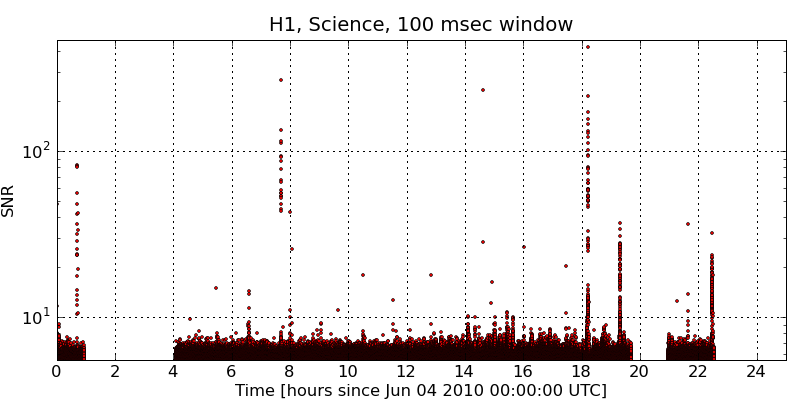
\includegraphics[width=0.5\linewidth]{figures/detchar/20100604_H1_0_100MILLISEC_CLUSTERED_snr_vs_time}
  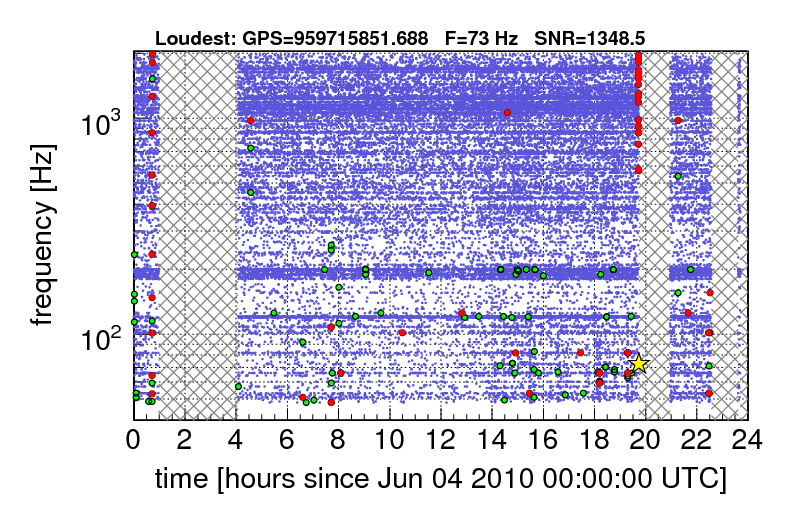
\includegraphics[width=0.5\linewidth]{figures/detchar/S6-H1-omega-959644815-959731215-GlitchTS}
  \caption[Use of daily ihope to indicate no veto needed] {
  \label{f:non_vetoed_time}
Use of daily ihope to indicate that time did not need to be vetoed.
The omega pipeline (left) shows a distinct feature at 200 Hz, within
the sensitive band of LIGO.  Daily ihope shows no excess of triggers
or SNR, and hence the time did not need to be vetoed}
\end{figure}%


\section{Applications of daily ihope to the blind injection challenge}
\label{sec:applications_applications_dog}


In addition to the hardware injections discussed in section
\ref{sec:ihope_hardware_injections} it was known at the start of S6
that there would be any from zero to ``a few'' unannounced, blind
hardware injections performed in order to provide an unbiased test of
the search pipelines.  One such injection was performed on Sep 16
2010 at 06:42 UTC, and showed up in multiple searches as a strong
gravitational wave candidate.  This candidate was followed up to the
point of writing a detection paper and submitting it to the
collaboration for publication approval.  Once approval had been
granted the fact that it had been an injection was revealed.  For more
details on the event and how it was followed up, see (the S6 low mass
paper).

Although daily ihope was not a search, the injection showed up on the
page of loudest triggers for H1 and L1, with parameters shown in table
\ref{tab:daily_ihope_dog} and omega scans shown in figure
\ref{f:daily_ihope_dog_omega}.  The injection was not visible in V1 in
daily ihope.

\begin{landscape}
\begin{table*}
\begin{center}
\begin{tabular}{lllllllllll}
\hline
ifo & end\_time & end\_time\_ns & SNR & $\chisq$ & New SNR & Mchirp & DQ flags \\
\hline
H1  & 968654557 & 997314453 & 15 & 87 & 9.8 & 4.6 & DMT-INSPIRAL\_RANGE\_STDEV\_GT\_0P50\_MPC \\
    &           &           &    &     &    &     & \hspace*{0.5 in} [968654544 968654560) \\
    &           &           &    &     &    &     & DMT-INSPIRAL\_RANGE\_STDEV\_GT\_0P75\_MPC \\
    &           &           &    &     &    &     & \hspace*{0.5 in} [968654544 968654560) \\
    &           &           &    &     &    &     & Light,Up,Calibrated,Science \\
\hline
L1 & 968654557 & 978027343 & 9.9 & 44 & 8.7 & 4.1 & SCI-OTHER\_ELOG [967120215 977875215) \\
    &           &           &    &     &    &     & DMT-INSPIRAL\_RANGE\_STDEV\_GT\_1\_MPC \\
    &           &           &    &     &    &     & \hspace*{0.5 in} [968654544 968654560) \\
    &           &           &    &     &    &     & DMT-INSPIRAL\_RANGE\_STDEV\_GT\_0P50\_MPC \\
    &           &           &    &     &    &     & \hspace*{0.5 in} [968654544 968654560) \\
    &           &           &    &     &    &     & DMT-INSPIRAL\_RANGE\_STDEV\_GT\_0P75\_MPC \\
    &           &           &    &     &    &     & \hspace*{0.5 in} [968654544 968654560) \\
    &           &           &    &     &    &     & SCI-FLAG\_ERROR \\
    &           &           &    &     &    &     & \hspace*{0.5 in} [967137346 977875215) \\
    &           &           &    &     &    &     & Light,Up,Calibrated,Science \\
\hline
\end{tabular}
\end{center}
  \caption[Recovered blind injection parameters]{
  \label{tab:daily_ihope_dog}
The blind injection as reported by daily ihope's ``loudest triggers'' page.}
\end{table*}
\end{landscape}


\begin{figure}
  \includegraphics[width=0.5\linewidth]{figures/detchar/968654557_997314453_H1_LSC-DARM_ERR_1_00_spectrogram_whitened.png}
  \includegraphics[width=0.5\linewidth]{figures/detchar/968654557_978027343_L1_LSC-DARM_ERR_1_00_spectrogram_whitened.png}
  \caption[Omega scans of the injection]{
  \label{f:daily_ihope_dog_omega}
H1 (left) and L1 (right) Omega scans of the injection as
generated by daily ihope.  Note the ``chirp'' shape which is the
expected pattern from a compact binary inspiral.}
\end{figure}%


\subsection{False Alarm Rate Estimate}

The potential detection occurred close to the end of S6 as the
collaboration was preparing to take the LIGO detectors apart 
to install advanced LIGO.  The shutdown could potentially have been
delayed if the existing configuration were necessary to vet
the candidate.  An ad-hoc committee was formed to determine whether
this would be required, and while they found no immediate reason to
delay the advanced LIGO plans the report did include several
recommendations, including:

% https://dcc.ligo.org/cgi-bin/private/DocDB/ShowDocument?docid=22752

\begin{quote}
The committee urges a search in the S6 and S5 data for events with
similar waveforms but lower SNR than the September 16 event in single
detectors as well as in dual detector coincidence. Such an
investigation has a dual purpose. First, it will establish some limits
on the astrophysical source population producing the September 16
event and second, it will help in estimating the false alarm rate,
although this will be better accomplished with more time
slides~\cite{Weiss:injection}.
\end{quote}

The existing daily ihope triggers were ideal for this purpose, as they
spanned all of S6 but with a reduced set of templates.  This sampled the
parameter space but produced a smaller set of triggers that made
rapid significance studies computationally feasible.

% https://www.lsc-group.phys.uwm.edu/ligovirgo/cbcnote/DailyDogHistograms

\iffalse
In order to determine the significance of this candidate event it was
necessary to compare it against the background.  The first such
comparison ranked the event against background triggers from the
two-week analysis in which it occurred as part of the standard ihope
pipeline.  However, the event had a larger combined new SNR value than
all background triggers, and hence had a false alarm probability of
zero.

In order to provide a more meaningful bound it was necessary to
increase the analysis time and/or number of slides to probe the
background more deeply. This is a complex and time-consuming process,
see (s6 paper) for details.  While this was underway we could begin to
bound the significance from daily ihope results.  This was done by
plotting histograms of all triggers throughout S6 and locating the
candidate triggers in the resulting distribution.  This analysis
differs from the full ihope pipeline in several respects.  However,
the goal was not a publishable result but only a rapid estimate.
\fi

The significance was estimated by plotting histograms of all triggers
throughout S6 and locating the candidate triggers in the resulting
distribution.  To parallel the full analysis the results were broken
into mass bins.  The low mass bin spans chirp masses up to
$3.48\msun$, the medium mass bin from $3.48-7.40 \msun$.  Likewise,
category 1,2 and 3 vetoes were applied to parallel the results of the
full search.  30-millisecond clustering was chosen to parallel the
clustering used in the full search.  There are several ways of
reporting the new SNR of the injection; the largest values reported by
daily ihope, the largest single-detector values reported by the full
search, and the component values of the largest combined new SNR
reported by the full search.  All of these options are included on the
plot.

The results are shown in figure \ref{f:daily_histogram_low} for the
low-mass bin and \ref{f:daily_histogram_medium} for the medium-mass
bin.  The result in both bins is qualitatively the same.  The
injection is close to the loudest event in H1 for all measures of new
SNR.  The injection does not stand out as far in L1, which was known
to be glitchier over the course of S6.


\begin{figure}
  \includegraphics[width=0.5\linewidth]{figures/detchar/LM_H1_30MILLISEC_3_hist.png}
  \includegraphics[width=0.5\linewidth]{figures/detchar/LM_L1_30MILLISEC_3_hist.png}
  \caption[Significance of the injection in the low-mass bin]{
  \label{f:daily_histogram_low}
Significance of the blind injection in the low-mass bin in H1 (left)
and L1 (right). Results are shown as cumulative histograms.  The plots
flatten out at low SNRs due the selection of triggers from the SNR
time series, discussed in
section~\ref{sec:analysis_trigger_selection}.  The red lines are the
new SNR reported by the full ihope run (after coincidence).  The green
lines are the loudest trigger in new SNR found at the first stage of
the ihope analysis (before coincidence).  The blue lines are the new
SNR values of the injection found by daily iHope (no coincidence).}
\end{figure}%



\begin{figure}
  \includegraphics[width=0.5\linewidth]{figures/detchar/MM_H1_30MILLISEC_3_hist.png}
  \includegraphics[width=0.5\linewidth]{figures/detchar/MM_L1_30MILLISEC_3_hist.png}
  \caption[Significance of the injection in the medium-mass bin]{
  \label{f:daily_histogram_medium}
Significance of the blind injection in the medium-mass bin in 
H1 (left) and L1 (right).  Note the cumulative counts levels off
around between 5 and 5.5, indicating that there are few triggers with
smaller values.}
\end{figure}%

\iffalse
From these results we can attempt to estimate a false alarm rate for
the injection as follows.   Model coincident triggers as a Bernoulli
trial where ``success'' is obtaining a coincidence with combined new
SNR greater than or equal to that of the injection.  Denote the
probability of success in a single trial as $P$.  Then the probability
of obtaining the first success after $k$ trials is a geometric
distribution, $Prob(k) = P(1-P)^{k-1}$, and the expected number of
trials before success is $1/P$.  Dividing this by the estimated number
of coincident triggers in a year gives the estimated number of years
required to obtain such a trigger by chance.

The rate of coincident triggers, $R$, in the full search was estimated
by choosing a few analysis chunks and dividing the number of H1L1
triggers by the analysis time, both of which are reported after the
coincidence step.  The average rate is approximately 0.004
coincidences per second of analysis time, or $N=126,144$ per year.
This is combined across all mass bins, the result will therefore be an
upper limit for any particular bin.

% CIT:
% /archive/home/sprivite/S6/lowmass/s6d_weeks33_34/968803143-970012887/full_data
% for i in `/bin/ls | grep H1L1-COIRE_FIRST_FULL_DATA `
% do
%  grep 'amount of time analysed' $i | cut -f7 -d' '
% done | awk '{s+=$1} END {print s}'
% 135254
%
% for i in `/bin/ls | grep H1L1-COIRE_FIRST_FULL_DATA `
% do
%  grep 'reconstructed' $i | cut -f7 -d' '
% done | awk '{s+=$1} END {print s}'
%
% 523
% so 523 / 135254 = 0.00387 coinc/sec
%
%
% LHO (dog)
% /archive/home/mtwest/CBC-s6d/weeks_31-32/lowmass_run/967593543-968803287/full_data
% Gives 
% 886 / 244515 = 0.00362 coinc/sec


We estimate $P$ by assuming a probability density function in each
detector of the form

\begin{equation}
P(\rho_\textrm{new}) = \left\{
  \begin{array}{lr}
    0  & \rho < 5.5 \\
    \exp\left(-\frac{\rho^2}{2\sigma^2}\right) & \rho_\textrm{new} \geq 5.5 \\
  \end{array} \right.
\end{equation}

The lower cutoff is approximate.  We do not threshold on new SNR, and
while we do threshold on$\rho > 5.5$ it is possible for $\chisq$ to
push the resulting new SNR down.  In addition, due to clustering, the
probability of obtaining low new SNR triggers is suppressed.  The fit
to the Gaussian portion of the curves is show on  figures
\ref{f:daily_histogram_low} and \ref{f:daily_histogram_medium}, and
the obtained values are shown in table \ref{tab:daily_ihope_sigmas}.

\begin{table*}
\begin{center}
\begin{tabular}{l | l l}
   & $\sigma_H$ & $\sigma_L$ \\
\hline
Low mass bin    & 0.98 & 0.96 \\
Medium mass bin & 0.99 & 0.97 \\
\end{tabular}
\end{center}
  \caption[Fit values for SNR histograms]{
  \label{tab:daily_ihope_sigmas}
$\sigma$ values obtained by fitting Gaussians to daily
ihope trigger counts.}
\end{table*}

The joint PDF is then

\begin{equation}
P(\rho_H,\rho_L) = \frac{1}{A}
\int_{\rho_L = 5.5}^{\sqrt{\rho_i^2 - \rho_L^2}}
\int_{\rho_H = 5.5}^{\sqrt{\rho_i^2 - 5.5^2}}
\exp\left(-\frac{\rho_H^2}{2\sigma^2}\right)
\exp\left(-\frac{\rho_L^2}{2\sigma^2}\right)
\,d\rho_H
\,d\rho_L
\end{equation}

where $A$ is the normalization obtained by taking the upper limits of
both integrals to infinity.  This may be simplified by means of the
substitutions

\begin{align*}
s      &= \frac{\rho_H}{\sqrt{2}\sigma_H} \\
s_{\mathrm{low}}  &= \frac{5.5}{\sqrt{2}\sigma_H} \\
s_{\mathrm{high}} &= \frac{\sqrt{\rho_i^2 - 5.5^2}}{\sqrt{2}\sigma_H} \\
t      &= \frac{\rho_L}{\sqrt{2}\sigma_L} \\
t_{\mathrm{low}}  &= \frac{5.5}{\sqrt{2}\sigma_L} \\
t_{\mathrm{high}}(s) &= \frac{\sqrt{\rho_i^2 - 2 \sigma_H^2 s^2}}{\sqrt{2}\sigma_L} \\
\end{align*}

in terms of which the normalization is

\begin{equation}
A = \frac{\pi}{2} \sigma_x \sigma_y \left[
1 - \erf(s_{\mathrm{low}}) - \erf(t_{\mathrm{low}}) + \erf(s_{\mathrm{low}})\erf(t_{\mathrm{low}})
\right]
\end{equation}

where $\erf$ is the error function.  The probability of obtaining a
trigger with combined new SNR larger than the injection is then

\begin{align*}
P &= 1 - \frac{\pi\sigma_L \sigma_H}{2 A} \bigg[
\frac{2}{\pi} \int_{s_{\mathrm{low}}}^{s_{\mathrm{high}}} e^{-s^2}
\erf(t_{\mathrm{high}}(s))\,ds \nonumber \\
&\quad - \erf(t_{\mathrm{low}}) \erf(s_{\mathrm{high}})  
+ \erf(s_{\mathrm{low}}) \erf (t_{\mathrm{low}}) \bigg] \\
\end{align*}


\iffalse
\begin{equation}
P(\rho_H,\rho_L) = 
\frac{4}{2\pi \sigma_H \sigma_L} 
\exp\left(
-\frac{\rho_H^2}{2\sigma_H^2} -\frac{\rho_L^2}{2\sigma_L^2}
\right)
\end{equation}

where the factor $4$ comes from considering only the quadrant where
both SNRs are positive.

The probability of obtaining a trigger with new SNR greater than
that of the injection, $\rho_i$, is then

\begin{equation}
P = 
\frac{4}{2\pi \sigma_H \sigma_L} 
\int_{\rho_H^2 + \rho_L^2 > \rho_i^2}
\exp\left(
-\frac{\rho_H^2}{2\sigma_H^2} -\frac{\rho_L^2}{2\sigma_L^2}
\right)
\,d\rho_H\,d\rho_L
\end{equation}

Introducing a temporary variable $M = \rho_L \sigma_H/\sigma_L$, going to polar
coordinates, evaluating the integral over $r$ and simplifying gives


\begin{equation}
P(\rho_c^2 > \rho_i^2|\textrm{coincidence}) = 
\frac{1}{2\pi \sigma_H \sigma_L} 
\frac{\sigma_L}{\sigma_H}
\int_{\rho_H^2 + (\sigma_L/\sigma_H)^2 M^2 \leq \rho_i^2}
\exp\left(
-\frac{\rho_H^2}{2\sigma_H^2} -\frac{M^2}{2\sigma_H^2}
\right)
\,d\rho_H\,dM
\end{equation}



\begin{equation}
P = 
\frac{1}{2\pi \sigma_H \sigma_L} 
\frac{\sigma_L}{\sigma_H}
\int_{r^2\cos^2\theta + (\sigma_L/\sigma_H)^2 r^2\sin^2\theta \leq \rho_i^2}
\exp\left(
-\frac{r^2\cos^2\theta}{2\sigma_H^2} -\frac{r^2\sin^2\theta}{2\sigma_H^2}
\right)
r\, dr\, d\theta
\end{equation}


\begin{equation}
P = 
\frac{1}{2\pi \sigma_H \sigma_L} 
\frac{\sigma_L}{\sigma_H}
\int_{r^2\cos^2\theta + (\sigma_L/\sigma_H)^2 r^2\sin^2\theta \leq \rho_i^2}
\exp\left( -\frac{r^2}{2\sigma_H^2} \right)
r\, dr\, d\theta
\end{equation}


\begin{equation}
P = 
\frac{1}{2\pi \sigma_H \sigma_L} 
\frac{\sigma_L}{\sigma_H}
\sigma_H^2
\int_0^{2\pi}
\left( 1 - 
\exp\left(
  -\frac{1}{2\sigma_H^2} 
   \frac{\rho_i^2}
        {\cos^2\theta + (\sigma_L/\sigma_H)^2 \sin^2\theta} 
\right)
\right)
d\theta
\end{equation}

\begin{equation}
P = \frac{4}{2\pi}
\int_0^{\pi/2}
\exp\left(
  -\frac{1}{2} 
   \frac{\rho_i^2}
        {\sigma_H^2 \cos^2\theta + \sigma_L^2 \sin^2\theta} 
\right)
d\theta
\end{equation}

\fi

This integral can be evaluated numerically.  Henceforth we focus on
the medium mass bin, as that was the bin with the most significant
trigger with a combined new SNR $\rho_i = 12.5$.  The result is
$P = 1.4 \times 10^{-20}$, which gives a false alarm rate of
1 event in 

\begin{equation}
\frac{1.0}{1.4 \times 10^{-26}} \times \frac{1}{126,144}
= 8.6\times 10^{24}\quad\textrm{years}
\end{equation}

This grossly underestimates the FAR calculated using time slides based
on the full analysis, which gives 1 in 7,000 years.  There is no
simple factor that explains this discrepancy; the two analyses are
significantly different that it is difficult to reason about the
results of the full analysis based on the output of single-stage
single-ifo triggers.  In particular the two-stage nature of the full
analysis introduces several complication.  However, this analysis does
suggest an alternative method to estimate FARs for a single-stage
pipeline which is currently in development.
\fi


\subsection{Front-end code verification}

% http://www.gravity.phy.syr.edu/dokuwiki/doku.php?id=larne:frontendcode
% https://dcc.ligo.org/cgi-bin/private/DocDB/ShowDocument?docid=39122
% https://dcc.ligo.org/cgi-bin/private/DocDB/ListBy?authorid=272

Before the collaboration could claim a detection it was necessary to
perform extensive checks to remove, or at least reduce, the
possibility that the trigger was due to any source other than a
gravitational wave.  Consequently many components of the
interferometer were subject to scrutiny.  One such component was the
\emph{front-end control code}, which is responsible for \Note{FILL
IN DETAILS}.  This code is updated occasionally as new systems are
added or bugs are found and fixed.   To verify that the most recent
change preceding the event did not significantly change the behavior
of the instruments we compared histograms of triggers from daily ihope
before and after these changes.

Two weeks prior to and following the most recent code changes at each
site were selected.  SNR histograms are shown in figure
\ref{f:code_changes}.  There is a slight variation in H1, somewhat
larger in L1.  More rigorous testing could have been done, such as
estimating the standard deviation in each SNR bin from several sample
times before the code change and then checking whether the rates after
the change fall within one sigma.  However, the detection committee
did not feel this level of analysis was necessary, and based on the
plots in figure \ref{f:code_changes} concluded:

\begin{figure}
  \includegraphics[width=0.5\linewidth]{figures/detchar/frontendtest_h1_log_2.png}
  \includegraphics[width=0.5\linewidth]{figures/detchar/frontendtest_l1_log_2.png}
  \caption[SNR histograms before and after code changes.] {
  \label{f:code_changes}
SNR histograms comparing periods before and after 
front-end code changes at H1 (left) and L1 (right).}
\end{figure}%

% https://dcc.ligo.org/cgi-bin/private/DocDB/ShowDocument?docid=39122

\begin{quote}
  Thus, to the extent allowed by the methods we adopted, there is no
  evidence for any malfunction in the front-end code of the
  interferometers~\cite{Whitcomb:injection}. 
\end{quote}



\section{Open Questions}
\label{sec:daily_ihope_open_questions}

Two potentially problematic features of the analysis were noticed in
daily ihope over the course of S6, both related to the effect of loud
glitches on the match filter.  Of course the ultimate goal is to
remove such glitches at the source.  However, it is likely that such
glitches will continue to be present in the advanced LIGO era and the
search pipeline must be robust against them.  We note here the
problems and some initial studies, but more research will be needed to
resolve them before advanced LIGO comes on-line around 2015.


\subsection{Excess triggers produced by loud glitches}
\label{ssec:penguins}

From figure~\ref{f:hepi_veto_effectiveness} we see that applying a
veto to loud glitches does not only remove loud triggers, but also
numerous triggers with lower SNRs.  This same effect may be seen by
comparing rate-vs-time and SNR-vs-time plots such
as~\ref{f:daily_ihope_grid}; loud glitches correlate with an increase
in trigger rates.  In part this behavior is expected.  Many glitches,
notably the spike glitch, are sharp enough that they may be roughly
modeled as impulses.  The impulse response of the match filter
(eqn.~\ref{eq:InnerProduct}) is the time-reversed template convolved
with a function of the noise curve.  A loud glitch will therefore
elevate the SNR time series for every template in the bank.

Recall from chapter~\ref{ch:search} that triggers are selected from
the SNR time series by finding the largest value above threshold in a
sliding window.  The length of the window is taken to the length of
the template, defined as the time required for the frequency of the pN
waveform to go from 40 Hz to infinity.  The selection is done using
the following algorithm: 

\begin{alltt}
for each sample point j
  if \(\rho\sb{j}\) > threshold
    if there is no event yet
      event\_start = j
      event\_snr   = \(\rho\sb{j}\)
    else if \(\rho\sb{j}\) > event\_snr
      event\_start = j
      event\_snr = \(\rho\sb{j}\)
    else if (j - event\_start) == template length
      record event
      event\_start = j
      event\_snr   = \(\rho\sb{j}\)
\end{alltt}

Based on this we would expect an impulse in the data to produce one
trigger per template at approximately the time of the impulse.
However this would not account for the number of templates seen or the
length of time for which the trigger rate is elevated. 

To study this in more detail simulated Gaussian noise was produced (as
in the NINJA project) and the value of a single sample was increased to
simulate a sharp glitch.  The triggers produced for two values of the
glitch amplitude are shown in
figure~\ref{f:impulses_original_no_chisq}.

\begin{figure}
  \includegraphics[width=0.5\linewidth]{figures/detchar/raw1_1e-17}
  \includegraphics[width=0.5\linewidth]{figures/detchar/raw1_1e-15}
  \caption[Response of the template bank to an impulse] {
  \label{f:impulses_original_no_chisq}
Trigger SNRs as a function of time as the template bank responds to an
impulse in the data.  Color is the length of the template in seconds.
On the left a single sample has been set to $10^{-17}$, and on the
right $10^{-15}$.  The expected response is visible, but there is a
large number of additional triggers arranged in distinct features.
See the text for discussion.
}
\end{figure}%

The expected behavior is seen in the rainbow ``tower'' at the top of
both plots, successively longer templates have lower SNRs and trigger
slightly later.

Below this in both plots there is a ``plateau'' of triggers from short
templates.  This results from the inverse spectrum truncation,
described more fully in~\cite{findchirp}.  This behavior can be
understood qualitatively as follows.

For simplicity denote the square root of the inverse PSD,
$(S_n(|f|))^{-1/2}$ as $\tilde{S}(f)$, and its inverse Fourier
transform in the time domain as $S(t)$.  Likewise, denote the
frequency-domain template as $\tilde{h}(f)$ as usual, and its inverse
Fourier transform as $h(t)$.  Finally, let $W(t)$ be a windowing
function in the time domain with Fourier transform $\tilde{W}(f)$.  In
addition, denote multiplication of function by $\cdot$ and convolution
by $\star$.

The application of the inverse spectrum truncation then proceeds as
follows 

1. Calculate $\tilde{S}(f)$ and from it $S(t)$.

2. Apply the window in the time domain, giving $S(t) \cdot W(t)$.

3. Return to to the frequency domain, giving $\tilde{S}(f) \star
\tilde{W}(f)$.

4. Square this (and correct the normalization, not shown here) giving 

\begin{equation*}
(\tilde{S}(f) \star \tilde{W}(f)) \cdot (\tilde{S}(f) \star \tilde{W}(f)) 
\end{equation*}

This replaces the $S_n(|f|)$ in the denominator of the match filter.

If the signal is then a delta function with strength $M$, $s(t) = M
\delta(t)$ then $\tilde{s} = M$  and the SNR time series the then
given by the matched filter,


\begin{align*}
\rho^2(t) &= \int df\, e^{-2 i\pi i f t} M \tilde{h}^\star(f) \cdot
(\tilde{S}(f) \star \tilde{W}(f)) \cdot 
(\tilde{S}(f) \star \tilde{W}(f)) \\
&= M h(-t) \star
(S(t) \cdot W(t)) \star
(s(t) \cdot w(t))
\end{align*}

Note that if the window function is zero outside a region then the
elevated SNR from an impulse will likewise be bounded in time.  This
is the motivation for the truncation; without it a loud glitch would
corrupt an entire analysis segment.  However, when $M$ becomes large
the SNR value within the bounded region may be sufficiently large to
exceed the trigger threshold.  If the length used when scanning the
SNR time series for triggers is less than the width of the truncation
window then a loud glitch can produce several triggers.  This explains
both the width of the plateaus in
figure~\ref{f:impulses_original_no_chisq} and why they are composed of
triggers from short templates.  This may also be seen in the SNR time
series shown in figure~\ref{f:short_snr_series}.

\begin{figure}
  \includegraphics[width=0.5\linewidth]{figures/detchar/snrs_17_short}
  \includegraphics[width=0.5\linewidth]{figures/detchar/snrs_15_short}
  \caption[SNR time series of a short template and loud impulse] {
The SNR time series of a short (0.3 s) template responding to an
impulse of strength $10^{-17}$ (left) and $10^{-15}$ (right).  The
elevation within the truncation window is clear, and is long enough to
produce several triggers.
  \label{f:short_snr_series}
}
\end{figure}%

The plateau persists as the strength of the impulse is increased.
Beyond a certain point we also get a second ``rainbow'' of triggers
from templates across the bank, seen to the right in
figure~\ref{f:impulses_original_no_chisq}.  Note that the difference
between triggers of the same color is precisely the length of
template, identified by the same value in the colorbar.  As the
impulse-response of the filter is the time-reversed template, a
sufficiently loud impulse will elevate the SNR for the length of the
template, independently of how the spectrum is truncated.   This can
be seen in the SNR time series of a long template, shown in
figure~\ref{f:long_snr_series}.


\begin{figure}
  \includegraphics[width=0.5\linewidth]{figures/detchar/snrs_17_long}
  \includegraphics[width=0.5\linewidth]{figures/detchar/snrs_15_long}
  \caption[SNR time series of a long template and loud impulse] {
  \label{f:long_snr_series}
The SNR time series of a long (45 s) template responding to an
impulse of strength $10^{-17}$ (left) and $10^{-15}$ (right).  The SNR
is elevated over the length of the template. \Note{TODO: triggers are
not lining up with the time series: check code.}
}
\end{figure}%

This second set of triggers from long templates suggests that the
length used when scanning the time series for is too short.  This,
combined with the excess of short triggers within the truncation
window suggests replacing this length with the larger of the length of
the truncation window or 1.1 times the currently used length (the
exact value to be obtained by further investigation).

So far we have not used the $\chisq$ test.  When $\chisq$ is
enabled the trigger clustering algorithm is modified as follows


\begin{alltt}
for each sample point j
  if \(\rho\sb{j}\) > threshold
    if \(\chisq\sb{j}\) < chisq\_thresh * (1 + \(\rho\sp{2}\) * chisqfac ):
      if there is no event yet
        event\_start = j
        event\_snr   = \(\rho\sb{j}\)
      else if \(\rho\sb{j}\) > event\_snr
        event\_start = j
        event\_snr = \(\rho\sb{j}\)
      else if (j - event\_start) == template length
        record event
        event\_start = j
        event\_snr   = \(\rho\sb{j}\)
\end{alltt}

That is, an additional constraint is placed on triggers even before
new SNR is calculated.  We would expect that this would quash many,
and hopefully all, triggers resulting from the glitch.  The results of
rerunning with $\chisq$ enabled are shown in
figure~\ref{f:impulses_original_chisq}.

\begin{figure}
  \includegraphics[width=0.5\linewidth]{figures/detchar/delta_chisq_1e-17}
  \includegraphics[width=0.5\linewidth]{figures/detchar/delta_chisq_1e-15}
  \caption[Triggers produced by loud impulses with $\chisq$ enabled] {
  \label{f:impulses_original_chisq}
Triggers produced by impulses of strength $10^{-17}$ (left) and
$10^{-15}$ (right) when the $\chisq$ test is enabled.  $\chisq$
removes many triggers, but many remain.
}
\end{figure}%

Turning on $\chisq$ does remove many triggers, in particular those in
the original tower resulting from long templates.  However, the
triggers from short templates remain.  This indicates that the
$\chisq$ test is not as effective on short waveforms, which is to be
expected.  The louder impulse on the right no longer produces the
second rainbow of triggers.  However, there are now long-template
triggers in the plateau, and a set of low-SNR, loud-template triggers
resulting from the quieter impulse.  The reason for these is not
clear, but they are have the potential to raise the background of the
binary neutron-star search and are therefore problematic.

Despite passing the $\chisq$ clustering it is unlikely that these
triggers, especially the ones from long templates, have good $\chisq$
values.  We can attempt to remove them by altering the clustering
algorithm as follows:


\begin{alltt}
for each sample point j
  if \(\rho\sb{j}\) > threshold
    if there is no event yet
      event\_start = j
      event\_snr   = \(\rho\sb{j}\)
    else if \(\rho\sb{j}\) > event\_snr
      event\_start = j
      event\_snr = \(\rho\sb{j}\)
    else if (j - event\_start) == template length
      if \(\chisq\sb{event_start}\) < chisq thresh * ( 1 + \(\rho\sp{2}\sb{event\_start}\) * chisqfac )
        record event
      event\_start = j
      event\_snr   = \(\rho\sb{j}\)
\end{alltt}

Rather than applying the $\chisq$ test at each sample point, we
cluster only on SNR and then use the $\chisq$ test to validate the 
candidate trigger.  This was implemented, along with altering the
clustering window as described above.  The results are shown in
Figure~\ref{f:impulses_new_chisq}, and appear very promising.  The
plateaus have been removed almost entirely, leaving only the last
trailing edge.  Only a few triggers from short templates remain, and
in particualr nothing that would interfere with the BNS search.

\begin{figure}
  \includegraphics[width=0.5\linewidth]{figures/detchar/1e-17_fixed_20100909}
  \includegraphics[width=0.5\linewidth]{figures/detchar/1e-15_fixed_20100909}
  \caption[Triggers produced by modified clustering algorithm] {
  \label{f:impulses_new_chisq}
Triggers produced by the modified clustering algorithm which extends
the clustering window and applies the $\chisq$  threshold after the
candidate trigger has been found.  Results are promising: only a
relatively small number of triggers from short templates remain.
}
\end{figure}%

The revised code was then tested by performing injections of simulated
signals into two weeks of real detector noise and examining the
numbers of injections found and missed.  The new code misses many more
injections, as shown in figure~\ref{f:found_missed_penguins}.  To see
why, consider a glitch with high SNR but high $\chisq$ within a
clustering window of an injection with lower SNR and lower $\chisq$.
In the original code the clustering window would not open at the
glitch, because it would not pass the $\chisq$ test.  The window would
open at the time of the injection, and the trigger would be recorded.
Under the new code, however, the higher SNR of the glitch will cause
it to be the single event found in the window, but it will then be
removed by the $\chisq$ test.  This problem is exacerbated by
extending the length of the window.

\begin{figure}
  \includegraphics[width=0.5\linewidth]{figures/detchar/penguin_foundmissed_orig}
  \includegraphics[width=0.5\linewidth]{figures/detchar/penguin_foundmissed_new}
  \caption[Found/missed plots showing the effect of new code] {
  \label{f:found_missed_penguins}
Found and missed plots for simulated injection in two weeks of real
noise.  Results from the current code are on the left, the modified
code (as described in the text) is on the right.  The feature to focus
on is found injections (blue dots) and missed injections (red
crosses).  There are many more missed injections using the modified
code.
}
\end{figure}%


At present the issue of excess triggers from loud glitches remains
unresolved.  It is mitigated somewhat by the ``loud SNR'' veto at
category 4, which extends $\pm 8$ seconds in order to remove the
excess triggers from the inverse spectrum truncation.  However, as
figure~\ref{f:impulses_original_no_chisq} shows, for very loud
glitches excess triggers can be produced for as much as 45.  An
appealing possibility that has been discussed but not tested would be
to run the current algorithm over a new SNR time series formed by
combining the SNR and $\chisq$ series.

\subsection{Bias of the PSD by loud glitches}
\label{ssec:sarlacc}

Loud glitches are often accompanied by surrounding periods of
decreased trigger rates, paradoxically.  This can be seen, for
example, in figure~\ref{f:daily_ihope_tcs}.  This effect is confined
to the 2048-second analysis segment containing the glitch, as can be
seen from figure~\ref{f:move_glitch}, which shows the trigger rate
around a glitch as the analysis boundaries are changed.

\begin{figure}
  \includegraphics[width=0.5\linewidth]{figures/detchar/H1-endtime_hist_ORIG}
  \includegraphics[width=0.5\linewidth]{figures/detchar/H1-endtime_hist_RESEG}
  \caption[Effect on trigger rates of a large glitch] {
  \label{f:move_glitch}
Effect on trigger rates of a large glitch.  The plots show the number
of triggers in an H1 analysis in 1-second blocks around a large glitch
centered at 2500.  The analysis boundaries are arranged so that on the
plot on the left the glitch falls at the end of the earlier segment,
while on the right the glitch falls at the beginning of the later
segment.  In both cases the glitch has the same number of triggers, 
which is well in excess of the surrounding time for reasons discussed
in the previous section.  However, the segment containing the glitch
shows a marked decrease in the number of triggers.
}
\end{figure}%

This behavior is due the effect of a glitch on the PSD estimation for
the analysis period.  Recall from chapter~\ref{ch:search} that the PSD
is estimated by Welch's method, and the value of the PSD at each
frequency $f$ is the median over 15 256-second intervals, overlapped
to span 2048 seconds.  The median is used instead of the mean
precisely because it is more robust against glitches.  However, a
values well outside the expected distribution can still bias the
results to a significant extent.  To demonstrate this we calculate the
PSD in two ways, once by considering the median of all 15 PSDs and
once by consider the median of 14, removing the one containing the 
glitch.  We plot the fractional difference of each frequency bin in
figure~\ref{f:median_bias}.


\begin{figure}
  \includegraphics[width=\linewidth]{figures/detchar/spectra_diffs}
  \caption[Bias in the PSD caused by a large glitch] {
  \label{f:median_bias}
The bias in the PSD caused by a large glitch.  This plot shows the
difference between two PSDs, one calculated including the
segment with the glitch and one without.  The results are shown as 
the fraction difference in each mass bin, (with - without) / with.
There is a notable bias upwards over much of the frequency range, and
in particular over the most sensitive portion of the LIGO band.
}
\end{figure}%

Some preliminary investigations using different-sized chunks and
overlaps to compute the PSD were performed, but these have so far been
inconclusive.  At present the only way to ensure that a loud glitch
won't suppress a quiet signal is to veto the time containing the
glitch at category 1.  This would be conceptually straightforward
using something like the existing category 4 ``loud SNR'' veto, but it
is far from an ideal solution.  This is especially true in advanced
LIGO, where the low-mass templates will be significantly longer.  A
glitch in the middle of such a signal could cause it to be lost, as
the category 1 veto would split the SNR accumulation into two disjoint
segments.   A better option would be to ``gate'' the data around a
glitch; smoothly window out a second or so with a Tukey window or
similar.  This is an area of ongoing research.

% tot_time, tot_count
% veto_time, veto_count

% $ ./check_flags.py L1
% 798720 2890507
%    880   12578
% $ ./check_flags.py H1
% 647168 1692904
%    416    6452


